% =====================================================================
% FAIR 2026 — báo cáo miệng 7 phút (bản tiếng Việt)
% Bài báo: papers/fair2026/manuscript/main_en.tex
% Bản gốc tiếng Anh: ../fair2026/main.tex — hai bản phải khớp số liệu
% Biên dịch: ./compile.sh   (XeLaTeX; bản kèm ghi chú: NOTES=1 ./compile.sh)
%
% Bản tiếng Việt chi tiết hơn bản tiếng Anh: thêm slide khử trùng lặp và
% thiết lập, rò rỉ cổng theo 8 thuật toán, TOST, hai chế độ F1 liên bộ và thích
% ứng miền. Số liệu vẫn phải khớp bài báo và bản tiếng Anh.
%
% KẾ HOẠCH THỜI GIAN (tổng ~11:00). Ba trang phân mục nằm giữa các phần, không
% được đánh số khung và mất ~5 s mỗi trang để bấm qua.
%   Trang bìa ...................... 0:20
%   I   Vấn đề, đóng góp ........... 1:30   (2 slide)
%   II  Quy trình, thiết lập ....... 2:00   (2 slide)
%   III Kết quả, kết luận .......... 7:00   (7 slide)
% Nếu chỉ có 7 phút: bỏ qua slide thiết lập, Kết quả 2 và Kết quả 6, chỉ nói
% câu kết luận của chúng.
% Sau slide tài liệu tham khảo là DỰ PHÒNG cho hỏi đáp.
% Ghi chú người trình bày nằm trong \note{} — dựng bằng NOTES=1.
% =====================================================================
\documentclass[aspectratio=169, 11pt]{beamer}
% =====================================================================
% Shared Beamer preamble for all decks in slides/
%   - 16:9, metropolis theme, Okabe-Ito colorblind-safe accents
%   - XeLaTeX + fontspec with a Vietnamese-capable sans fallback chain
%   - Speaker notes: compile with \def\shownotes{} to get the notes PDF
% Input this file right after \documentclass in each deck.
% =====================================================================

\usetheme{metropolis}
\metroset{block=fill, numbering=fraction, progressbar=frametitle, sectionpage=progressbar}

\usepackage{fontspec}
\usepackage{graphicx}
\usepackage{booktabs}
\usepackage{multirow}
\usepackage{amsmath,amssymb}
\usepackage{xcolor}
\usepackage{tikz}
\usetikzlibrary{positioning, arrows.meta, shapes.geometric, fit, backgrounds, calc}
\usepackage{appendixnumberbeamer}

% ---------------------------------------------------------------------
% Fonts. TeX Gyre Heros is the portable first choice (ships with a full
% TeX Live and covers Vietnamese); on a BasicTeX/macOS box it is absent,
% so fall back to system sans fonts that still carry Vietnamese
% diacritics, and only as a last resort to the serif TeX Gyre Termes
% (which is always present) rather than silently hitting nullfont.
% ---------------------------------------------------------------------
\IfFontExistsTF{TeX Gyre Heros}
  {\setsansfont{TeX Gyre Heros}[Ligatures=TeX]}
  {\IfFontExistsTF{Helvetica Neue}
     {\setsansfont{Helvetica Neue}[Ligatures=TeX]}
     {\IfFontExistsTF{Arial}
        {\setsansfont{Arial}[Ligatures=TeX]}
        {\setsansfont{TeX Gyre Termes}[Ligatures=TeX]}}}
\IfFontExistsTF{Menlo}
  {\setmonofont{Menlo}[Scale=0.82]}
  {\IfFontExistsTF{TeX Gyre Cursor}{\setmonofont{TeX Gyre Cursor}[Scale=0.85]}{}}

% ---------------------------------------------------------------------
% Palette. Blue and green follow the Okabe-Ito accents used in the
% manuscript TikZ figures; the emphasis accent is a red rather than
% Okabe-Ito's vermillion, so highlighted numbers read unambiguously as
% "look here" from the back of the room.
% ---------------------------------------------------------------------
\definecolor{accBlue}{HTML}{0072B2}
\definecolor{accGreen}{HTML}{009E73}
\definecolor{accRed}{HTML}{C1121F}
\definecolor{inkDark}{HTML}{23373B}

\setbeamercolor{frametitle}{bg=accBlue, fg=white}
\setbeamercolor{progress bar}{fg=accRed, bg=accRed!25}
\setbeamercolor{progress bar in head/foot}{fg=accRed, bg=accBlue!25}
\setbeamercolor{progress bar in section page}{fg=accRed, bg=accRed!25}
\setbeamercolor{alerted text}{fg=accRed}
\setbeamercolor{example text}{fg=accGreen}
\setbeamercolor{block title}{bg=accBlue!12, fg=inkDark}
\setbeamercolor{block body}{bg=accBlue!5}
\setbeamercolor{block title alerted}{bg=accRed!15, fg=inkDark}
\setbeamercolor{block body alerted}{bg=accRed!6}
\setbeamercolor{block title example}{bg=accGreen!15, fg=inkDark}
\setbeamercolor{block body example}{bg=accGreen!6}

% [standout] frames: metropolis paints them dark teal. Use the same blue as
% the frame titles so the closing slide reads as part of the same deck, and
% size the text up — it is meant to be seen from the back of the room.
\setbeamercolor{palette primary}{bg=accBlue, fg=white}
\setbeamerfont{standout}{size=\huge, series=\bfseries}

% Metropolis draws no bullet glyph by default; a small square reads better
% from the back of a conference room than pure indentation.
\setbeamertemplate{itemize item}{\raisebox{0.12ex}{\tiny$\blacksquare$}}
\setbeamertemplate{itemize subitem}{\raisebox{0.12ex}{\tiny$\square$}}
\setbeamercolor{itemize item}{fg=accBlue}
\setbeamercolor{itemize subitem}{fg=accBlue!70}

% Vietnamese has few hyphenation points, so a long run of words can fail to
% break and stick out past the text block. Allow looser interword glue as a
% last resort instead of an overfull line.
\setlength{\emergencystretch}{2em}

% Tables: booktabs rules look thin on a projector.
\setlength{\heavyrulewidth}{1.1pt}
\setlength{\lightrulewidth}{0.6pt}
\renewcommand{\arraystretch}{1.15}

% ---------------------------------------------------------------------
% Centre the title page and the section pages. Metropolis left-aligns both
% (\raggedright inside its templates); all three decks here want them
% centred, so each calls \centeredtitles right after loading this file.
% It stays a macro rather than an unconditional override so a future deck
% can keep the stock metropolis alignment by simply not calling it.
% ---------------------------------------------------------------------
\makeatletter
\newcommand{\centeredtitles}{%
  % Applied through \AtBeginDocument: metropolis re-applies its own inner
  % templates at \begin{document}, so overrides installed earlier are
  % silently reverted.
  \AtBeginDocument{%
    % Metropolis' title page puts the title graphic in a \vbox to 0pt at the
    % very top of a bottom-aligned \paperheight minipage — the image loads but
    % lands off the top of the page. Rebuild the title page with the graphic
    % after the opening \vfill, where it is actually visible.
    \setbeamertemplate{title graphic}{}%
    \setbeamertemplate{title page}{%
      \begin{minipage}[b][\paperheight]{\textwidth}
        \vfill
        \centering
        \ifx\inserttitlegraphic\@empty\else
          \inserttitlegraphic\par\vspace*{1.1em}%
        \fi
        \ifx\inserttitle\@empty\else\usebeamertemplate*{title}\fi
        \ifx\insertsubtitle\@empty\else\usebeamertemplate*{subtitle}\fi
        \usebeamertemplate*{title separator}
        \ifx\beamer@shortauthor\@empty\else\usebeamertemplate*{author}\fi
        \ifx\insertdate\@empty\else\usebeamertemplate*{date}\fi
        \ifx\insertinstitute\@empty\else\usebeamertemplate*{institute}\fi
        \vfill
        \vspace*{1mm}
      \end{minipage}}%
    \setbeamertemplate{title}{%
      \centering\linespread{1.0}\inserttitle\par\vspace*{0.5em}}%
    \setbeamertemplate{subtitle}{%
      \centering\insertsubtitle\par\vspace*{0.5em}}%
    \setbeamertemplate{author}{%
      \vspace*{2em}\centering\insertauthor\par\vspace*{0.25em}}%
    \setbeamertemplate{date}{%
      \centering\insertdate\par}%
    \setbeamertemplate{institute}{%
      \vspace*{3mm}\centering\insertinstitute\par}%
    % Same as metropolis' "progressbar" section page, but centred. No deck
    % here uses subsections, so that branch of the original is dropped.
    \setbeamertemplate{section page}{%
      \centering
      \begin{minipage}{22em}
        \centering
        \usebeamercolor[fg]{section title}%
        \usebeamerfont{section title}%
        \insertsectionhead\\[-1ex]
        \usebeamertemplate*{progress bar in section page}%
        \par
      \end{minipage}
      \par
      \vspace{\baselineskip}}%
  }%
}
\makeatother

% Shrink a box to the available width, but only when it would otherwise
% overflow. A tabular that is wider than its beamer column is NOT clipped —
% it silently overprints the neighbouring column — so every table that sits
% inside \begin{columns} goes through this.
\newcommand{\fitwidth}[1]{%
  \resizebox{\ifdim\width>\linewidth\linewidth\else\width\fi}{!}{#1}}

% ---------------------------------------------------------------------
% Emphasis macros used throughout the decks.
% ---------------------------------------------------------------------
\newcommand{\key}[1]{\textcolor{accBlue}{\textbf{#1}}}
\newcommand{\good}[1]{\textcolor{accGreen}{\textbf{#1}}}
\newcommand{\bad}[1]{\textcolor{accRed}{\textbf{#1}}}
\newcommand{\num}[1]{\textcolor{accRed}{\textbf{#1}}}

% One-line "so what" strip, pinned at the bottom of a result slide.
% Kept deliberately compact: this box sits directly above metropolis' frame
% number, so any extra height here pushes text into the footer and the page
% number ends up printed on top of the last line.
\newcommand{\takeaway}[1]{%
  \vfill
  \begin{beamercolorbox}[wd=\textwidth, sep=4pt, rounded=true]{block body example}%
    \footnotesize #1%
  \end{beamercolorbox}}

% ---------------------------------------------------------------------
% Speaker notes. Build the plain deck normally; build the notes version
% with:  xelatex "\def\shownotes{}% =====================================================================
% FAIR 2026 — báo cáo miệng 7 phút (bản tiếng Việt)
% Bài báo: papers/fair2026/manuscript/main_en.tex
% Bản gốc tiếng Anh: ../fair2026/main.tex — hai bản phải khớp số liệu
% Biên dịch: ./compile.sh   (XeLaTeX; bản kèm ghi chú: NOTES=1 ./compile.sh)
%
% Bản tiếng Việt chi tiết hơn bản tiếng Anh: thêm slide khử trùng lặp và
% thiết lập, rò rỉ cổng theo 8 thuật toán, TOST, hai chế độ F1 liên bộ và thích
% ứng miền. Số liệu vẫn phải khớp bài báo và bản tiếng Anh.
%
% KẾ HOẠCH THỜI GIAN (tổng ~11:00). Ba trang phân mục nằm giữa các phần, không
% được đánh số khung và mất ~5 s mỗi trang để bấm qua.
%   Trang bìa ...................... 0:20
%   I   Vấn đề, đóng góp ........... 1:30   (2 slide)
%   II  Quy trình, thiết lập ....... 2:00   (2 slide)
%   III Kết quả, kết luận .......... 7:00   (7 slide)
% Nếu chỉ có 7 phút: bỏ qua slide thiết lập, Kết quả 2 và Kết quả 6, chỉ nói
% câu kết luận của chúng.
% Sau slide tài liệu tham khảo là DỰ PHÒNG cho hỏi đáp.
% Ghi chú người trình bày nằm trong \note{} — dựng bằng NOTES=1.
% =====================================================================
\documentclass[aspectratio=169, 11pt]{beamer}
% =====================================================================
% Shared Beamer preamble for all decks in slides/
%   - 16:9, metropolis theme, Okabe-Ito colorblind-safe accents
%   - XeLaTeX + fontspec with a Vietnamese-capable sans fallback chain
%   - Speaker notes: compile with \def\shownotes{} to get the notes PDF
% Input this file right after \documentclass in each deck.
% =====================================================================

\usetheme{metropolis}
\metroset{block=fill, numbering=fraction, progressbar=frametitle, sectionpage=progressbar}

\usepackage{fontspec}
\usepackage{graphicx}
\usepackage{booktabs}
\usepackage{multirow}
\usepackage{amsmath,amssymb}
\usepackage{xcolor}
\usepackage{tikz}
\usetikzlibrary{positioning, arrows.meta, shapes.geometric, fit, backgrounds, calc}
\usepackage{appendixnumberbeamer}

% ---------------------------------------------------------------------
% Fonts. TeX Gyre Heros is the portable first choice (ships with a full
% TeX Live and covers Vietnamese); on a BasicTeX/macOS box it is absent,
% so fall back to system sans fonts that still carry Vietnamese
% diacritics, and only as a last resort to the serif TeX Gyre Termes
% (which is always present) rather than silently hitting nullfont.
% ---------------------------------------------------------------------
\IfFontExistsTF{TeX Gyre Heros}
  {\setsansfont{TeX Gyre Heros}[Ligatures=TeX]}
  {\IfFontExistsTF{Helvetica Neue}
     {\setsansfont{Helvetica Neue}[Ligatures=TeX]}
     {\IfFontExistsTF{Arial}
        {\setsansfont{Arial}[Ligatures=TeX]}
        {\setsansfont{TeX Gyre Termes}[Ligatures=TeX]}}}
\IfFontExistsTF{Menlo}
  {\setmonofont{Menlo}[Scale=0.82]}
  {\IfFontExistsTF{TeX Gyre Cursor}{\setmonofont{TeX Gyre Cursor}[Scale=0.85]}{}}

% ---------------------------------------------------------------------
% Palette. Blue and green follow the Okabe-Ito accents used in the
% manuscript TikZ figures; the emphasis accent is a red rather than
% Okabe-Ito's vermillion, so highlighted numbers read unambiguously as
% "look here" from the back of the room.
% ---------------------------------------------------------------------
\definecolor{accBlue}{HTML}{0072B2}
\definecolor{accGreen}{HTML}{009E73}
\definecolor{accRed}{HTML}{C1121F}
\definecolor{inkDark}{HTML}{23373B}

\setbeamercolor{frametitle}{bg=accBlue, fg=white}
\setbeamercolor{progress bar}{fg=accRed, bg=accRed!25}
\setbeamercolor{progress bar in head/foot}{fg=accRed, bg=accBlue!25}
\setbeamercolor{progress bar in section page}{fg=accRed, bg=accRed!25}
\setbeamercolor{alerted text}{fg=accRed}
\setbeamercolor{example text}{fg=accGreen}
\setbeamercolor{block title}{bg=accBlue!12, fg=inkDark}
\setbeamercolor{block body}{bg=accBlue!5}
\setbeamercolor{block title alerted}{bg=accRed!15, fg=inkDark}
\setbeamercolor{block body alerted}{bg=accRed!6}
\setbeamercolor{block title example}{bg=accGreen!15, fg=inkDark}
\setbeamercolor{block body example}{bg=accGreen!6}

% [standout] frames: metropolis paints them dark teal. Use the same blue as
% the frame titles so the closing slide reads as part of the same deck, and
% size the text up — it is meant to be seen from the back of the room.
\setbeamercolor{palette primary}{bg=accBlue, fg=white}
\setbeamerfont{standout}{size=\huge, series=\bfseries}

% Metropolis draws no bullet glyph by default; a small square reads better
% from the back of a conference room than pure indentation.
\setbeamertemplate{itemize item}{\raisebox{0.12ex}{\tiny$\blacksquare$}}
\setbeamertemplate{itemize subitem}{\raisebox{0.12ex}{\tiny$\square$}}
\setbeamercolor{itemize item}{fg=accBlue}
\setbeamercolor{itemize subitem}{fg=accBlue!70}

% Vietnamese has few hyphenation points, so a long run of words can fail to
% break and stick out past the text block. Allow looser interword glue as a
% last resort instead of an overfull line.
\setlength{\emergencystretch}{2em}

% Tables: booktabs rules look thin on a projector.
\setlength{\heavyrulewidth}{1.1pt}
\setlength{\lightrulewidth}{0.6pt}
\renewcommand{\arraystretch}{1.15}

% ---------------------------------------------------------------------
% Centre the title page and the section pages. Metropolis left-aligns both
% (\raggedright inside its templates); all three decks here want them
% centred, so each calls \centeredtitles right after loading this file.
% It stays a macro rather than an unconditional override so a future deck
% can keep the stock metropolis alignment by simply not calling it.
% ---------------------------------------------------------------------
\makeatletter
\newcommand{\centeredtitles}{%
  % Applied through \AtBeginDocument: metropolis re-applies its own inner
  % templates at \begin{document}, so overrides installed earlier are
  % silently reverted.
  \AtBeginDocument{%
    % Metropolis' title page puts the title graphic in a \vbox to 0pt at the
    % very top of a bottom-aligned \paperheight minipage — the image loads but
    % lands off the top of the page. Rebuild the title page with the graphic
    % after the opening \vfill, where it is actually visible.
    \setbeamertemplate{title graphic}{}%
    \setbeamertemplate{title page}{%
      \begin{minipage}[b][\paperheight]{\textwidth}
        \vfill
        \centering
        \ifx\inserttitlegraphic\@empty\else
          \inserttitlegraphic\par\vspace*{1.1em}%
        \fi
        \ifx\inserttitle\@empty\else\usebeamertemplate*{title}\fi
        \ifx\insertsubtitle\@empty\else\usebeamertemplate*{subtitle}\fi
        \usebeamertemplate*{title separator}
        \ifx\beamer@shortauthor\@empty\else\usebeamertemplate*{author}\fi
        \ifx\insertdate\@empty\else\usebeamertemplate*{date}\fi
        \ifx\insertinstitute\@empty\else\usebeamertemplate*{institute}\fi
        \vfill
        \vspace*{1mm}
      \end{minipage}}%
    \setbeamertemplate{title}{%
      \centering\linespread{1.0}\inserttitle\par\vspace*{0.5em}}%
    \setbeamertemplate{subtitle}{%
      \centering\insertsubtitle\par\vspace*{0.5em}}%
    \setbeamertemplate{author}{%
      \vspace*{2em}\centering\insertauthor\par\vspace*{0.25em}}%
    \setbeamertemplate{date}{%
      \centering\insertdate\par}%
    \setbeamertemplate{institute}{%
      \vspace*{3mm}\centering\insertinstitute\par}%
    % Same as metropolis' "progressbar" section page, but centred. No deck
    % here uses subsections, so that branch of the original is dropped.
    \setbeamertemplate{section page}{%
      \centering
      \begin{minipage}{22em}
        \centering
        \usebeamercolor[fg]{section title}%
        \usebeamerfont{section title}%
        \insertsectionhead\\[-1ex]
        \usebeamertemplate*{progress bar in section page}%
        \par
      \end{minipage}
      \par
      \vspace{\baselineskip}}%
  }%
}
\makeatother

% Shrink a box to the available width, but only when it would otherwise
% overflow. A tabular that is wider than its beamer column is NOT clipped —
% it silently overprints the neighbouring column — so every table that sits
% inside \begin{columns} goes through this.
\newcommand{\fitwidth}[1]{%
  \resizebox{\ifdim\width>\linewidth\linewidth\else\width\fi}{!}{#1}}

% ---------------------------------------------------------------------
% Emphasis macros used throughout the decks.
% ---------------------------------------------------------------------
\newcommand{\key}[1]{\textcolor{accBlue}{\textbf{#1}}}
\newcommand{\good}[1]{\textcolor{accGreen}{\textbf{#1}}}
\newcommand{\bad}[1]{\textcolor{accRed}{\textbf{#1}}}
\newcommand{\num}[1]{\textcolor{accRed}{\textbf{#1}}}

% One-line "so what" strip, pinned at the bottom of a result slide.
% Kept deliberately compact: this box sits directly above metropolis' frame
% number, so any extra height here pushes text into the footer and the page
% number ends up printed on top of the last line.
\newcommand{\takeaway}[1]{%
  \vfill
  \begin{beamercolorbox}[wd=\textwidth, sep=4pt, rounded=true]{block body example}%
    \footnotesize #1%
  \end{beamercolorbox}}

% ---------------------------------------------------------------------
% Speaker notes. Build the plain deck normally; build the notes version
% with:  xelatex "\def\shownotes{}\input{main.tex}"
% ---------------------------------------------------------------------
\ifdefined\shownotes
  \usepackage{pgfpages}
  \setbeameroption{show notes on second screen=right}
\fi

\centeredtitles

\graphicspath{%
  {../../results/ml_07_cross_method_comparison/}%
  {../../results/ml_05_shap_explainability/}%
  {../../results/ml_06_feature_selection_shap/}%
  {../../results/ml_09_multiclass_eval/}%
  {../../results/ml_10_leakage_ablation/}%
  {../../results/ml_11_cross_dataset/}%
}

\title{Giảm chiều và chọn lọc đặc trưng cho phát hiện xâm nhập mạng trên Apache Spark ML}
\subtitle{\ldots với quy trình đánh giá loại rò rỉ dữ liệu}
\author{\textbf{Nguyễn Vũ Thái}\inst{1} \and Bùi Văn Dũng\inst{2} \and Đỗ Trí Nhựt\inst{2} \and Nguyễn Văn Dũ\inst{3}}
\institute{\scriptsize
           \inst{1}Phân hiệu tại TP.\ Hồ Chí Minh, Trường Đại học Giao thông Vận tải, TP.\ Hồ Chí Minh, Việt Nam \\
           \inst{2}Trường Đại học Công nghệ Thông tin, ĐHQG-HCM, TP.\ Hồ Chí Minh, Việt Nam \\
           \inst{3}Khoa Công nghệ Thông tin, Trường Đại học Nông Lâm, TP.\ Hồ Chí Minh, Việt Nam}
\date{FAIR'2026}

\begin{document}

% ---------------------------------------------------------------- 0:20
\maketitle
\note{Bảy phút cho một luận điểm duy nhất: trên CICIDS2017, F1 gần như hoàn hảo
thường là tính chất của quy trình đánh giá, không phải của mô hình.}

% ---------------------------------------------------------------- 0:50
% =====================================================================
\section{I.\ VẤN ĐỀ VÀ ĐÓNG GÓP}
% =====================================================================

\begin{frame}{F1 gần như hoàn hảo trên CICIDS2017 là một dấu hiệu đáng ngờ}
  \begin{columns}[T]
    \begin{column}{0.55\textwidth}
      \textbf{Hai vấn đề, thường được xét riêng}
      \begin{itemize}
        \item \key{Chi phí.} $\approx$80 đặc trưng mỗi luồng.
        \item \key{Độ tin cậy.} F1 nhị phân gần hoàn hảo thường báo hiệu
              \bad{rò rỉ dữ liệu}.
      \end{itemize}
      \vspace{0.5em}
      \textbf{Hai nguồn rò rỉ cụ thể}
      \begin{enumerate}
        \item \texttt{destination\_port} mã hóa \emph{dịch vụ bị tấn công}.
        \item \bad{Trùng lặp ở mức đặc trưng} sống sót qua khử trùng lặp
              toàn dòng --- cùng một mẫu nằm ở \emph{cả} tập huấn luyện
              \emph{và} tập kiểm tra.
      \end{enumerate}
    \end{column}
    \begin{column}{0.42\textwidth}
      \begin{alertblock}{Bài báo này}
        So sánh bốn chiến lược giảm chiều trên cùng tám bộ phân loại Spark ML
        --- nhưng trước hết làm cho \emph{quy trình đánh giá} đáng tin đã.
      \end{alertblock}
      \begin{exampleblock}{Đóng góp nằm ở giao thức đo}
        Không phải ``phương pháp nào thắng'' mà là \key{đo thế nào để câu trả
        lời có ý nghĩa}.
      \end{exampleblock}%
    \end{column}
  \end{columns}
  \note{Rò rỉ dữ liệu: thông tin không có lúc triển khai lọt vào huấn luyện hoặc
  đánh giá. Định vị bài báo là bài về phép đo. Cổng đích cho mô hình một đường tắt
  từ cổng sang nhãn; 80 đặc trưng thì tốn cả khi huấn luyện, khi suy luận và
  khi nhồi lên thiết bị biên. Cả hai nguồn rò rỉ đều được loại trước khi chia
  tập.}
\end{frame}

% ---------------------------------------------------------------- 0:35
\begin{frame}{Các đóng góp}
  \begin{enumerate}
    \item \key{So sánh thống nhất} giữa RF Importance, SHAP và PCA trên cùng 8
          thuật toán Spark ML $+$ 2 mô hình tổ hợp, trên CICIDS2017.
    \item SHAP được đặt \key{trực tiếp} cạnh RF Importance trên cùng tập huấn
          luyện.
    \item Quy trình \key{loại rò rỉ và có kiểm định thống kê}: loại đặc trưng rò
          rỉ, khử trùng lặp ở mức đặc trưng một cách tất định, chọn mô hình trên
          tập kiểm định, kiểm định hoán vị ghép cặp liệt kê đầy đủ kèm hiệu chỉnh
          Nadeau--Bengio.
    \item \key{Đánh giá đa lớp theo từng loại tấn công} --- nơi các phương pháp
          thực sự khác nhau.
    \item Khuyến nghị \key{có tính tới thiết bị biên}: F1 \emph{và} số đặc trưng
          \emph{và} kích thước mô hình, cho Jetson Orin Nano Super (phần triển
          khai nằm ở một bài hệ thống đi kèm).
  \end{enumerate}
  \note{Năm đóng góp; ba, bốn và năm là những thứ ít khi được làm cùng nhau.}
\end{frame}

% ---------------------------------------------------------------- 0:55
% =====================================================================
\section{II.\ QUY TRÌNH LOẠI RÒ RỈ}
% =====================================================================

\begin{frame}{Quy trình loại rò rỉ}
  \begin{columns}[c]
    \begin{column}{0.5\textwidth}
      \centering
      \resizebox{0.98\textwidth}{!}{%
      \begin{tikzpicture}[
        font=\footnotesize, node distance=2.6mm, >=Stealth,
        box/.style={draw=gray!60, rounded corners=2pt, align=center, inner sep=4pt, minimum width=7.6cm},
        hl/.style={box, draw=accRed, fill=accRed!10},
        ed/.style={box, draw=accGreen!80!black, fill=accGreen!10},
        arr/.style={-{Stealth[length=2mm]}, semithick}]
        \node[box] (raw)  {CICIDS2017 --- 8 tệp CSV, $\approx$2,8 triệu luồng};
        \node[hl, below=of raw] (prep) {\textbf{Chuẩn bị dữ liệu loại rò rỉ}\\
              loại \texttt{destination\_port} $\cdot$ khử trùng lặp mức đặc trưng};
        \node[box, below=of prep] (split) {Chia 80/20 (hạt giống cố định) $\cdot$ Parquet};
        \node[box, below=of split] (strat) {\textbf{4 chiến lược}: Cơ sở $|$ RF Top-$K$ $|$ SHAP Top-$K$ $|$ PCA\\
              (xếp hạng khớp \emph{chỉ trên tập huấn luyện})};
        \node[box, below=of strat] (clf) {8 bộ phân loại Spark ML $+$ 2 tổ hợp};
        \node[hl, below=of clf] (val) {Chọn mô hình trên tập kiểm định $\cdot$ kiểm định hoán vị ghép cặp\\
              khoảng tin cậy Nadeau--Bengio $\cdot$ cỡ hiệu ứng $\cdot$ đa lớp};
        \node[ed, below=of val] (edge) {SHAP Top-30 $\rightarrow$ Jetson Orin Nano Super};
        \draw[arr] (raw)--(prep); \draw[arr] (prep)--(split); \draw[arr] (split)--(strat);
        \draw[arr] (strat)--(clf); \draw[arr] (clf)--(val); \draw[arr] (val)--(edge);
      \end{tikzpicture}}
    \end{column}
    \begin{column}{0.47\textwidth}
      \textbf{Mỗi bước chặn một đường rò rỉ}
      \begin{itemize}\footnotesize
        \item Loại cổng đích: chặn \bad{đường tắt cổng $\to$ nhãn}.
        \item Khử trùng lặp \emph{trước} khi chia: không mẫu nào ở cả hai tập.
        \item Scaler, PCA, xếp hạng RF/SHAP chỉ \emph{fit} trên tập huấn luyện.
        \item Chọn mô hình trên tập kiểm định (20\% tập huấn luyện): tập kiểm
              tra \bad{không} tham gia bước chọn nào.
      \end{itemize}
      \vspace{0.2em}
      \textbf{Thiết kế cố định \emph{từ trước}}
      \begin{itemize}\footnotesize
        \item Quét $K \in \{20,30,40\}$ tách khỏi pha xác nhận 4 cấu hình:
              Cơ sở, RF Top-30, SHAP Top-30, PCA $k{=}40$.
      \end{itemize}
    \end{column}
  \end{columns}
  \note{Đi từ trên xuống, mỗi khối đỏ là một chỗ rò rỉ bị chặn. Không cấu hình
  nào được chọn theo F1 trên tập kiểm tra. Siêu tham số dùng chung cho mọi
  phương pháp, nên khác biệt phản ánh phương pháp chứ không phải việc tinh
  chỉnh.}
\end{frame}

% ---------------------------------------------------------------- 1:05
\begin{frame}{Khử trùng lặp tất định và thiết lập thực nghiệm}
  \begin{columns}[T]
    \begin{column}{0.52\textwidth}
      \textbf{Chuẩn bị dữ liệu, trước khi chia tập}
      \begin{enumerate}\footnotesize
        \item Gộp 8 tệp CSV; $\pm\infty \to$ NaN; bỏ dòng thiếu, dòng trùng.
        \item Nhãn: BENIGN $\to 0$, mọi tấn công $\to 1$.
        \item Đặc trưng $\mathcal{F}$: cột số, \emph{trừ} cổng, giao thức,
              định danh.
        \item Nhóm dòng giống hệt nhau trên $\mathcal{F}$:
              mâu thuẫn nhãn $\to$ \bad{loại cả nhóm}
              (\num{270 nhóm, 44.260 dòng}); còn lại $\to$ giữ \emph{một}
              đại diện tất định.
        \item Chia 80/20, hạt giống cố định.
      \end{enumerate}
    \end{column}
    \begin{column}{0.45\textwidth}
      \centering\scriptsize
      \fitwidth{%
      \begin{tabular}{lr}
        \toprule
        \multicolumn{2}{l}{\textbf{CICIDS2017} (sau xử lý)} \\
        \midrule
        Đặc trưng số             & 77 \\
        Huấn luyện / kiểm tra    & 1.785.349 / 447.275 \\
        Tổng                     & 2.232.624 \\
        \midrule
        \multicolumn{2}{l}{\textbf{CSE-CIC-IDS2018} (mẫu phân tầng 20\%)} \\
        \midrule
        Trước / sau khử trùng lặp & $\sim$3,14 / $\sim$2,39 triệu \\
        \bottomrule
      \end{tabular}
      }
      \vspace{0.4em}

      \raggedright
      \begin{itemize}\scriptsize
        \item \textbf{Hạ tầng:} Spark 3.4.1; 2$\times$ Jetson Orin Nano Super
              (8\,GB) làm worker, máy chủ \emph{chỉ} làm master.
        \item \textbf{Chỉ số:} ưu tiên \key{AUC-PR} và \key{recall tấn công}
              hơn accuracy vì dữ liệu mất cân bằng.
        \item Mã nguồn công khai; chạy lại được trên một máy.
      \end{itemize}
    \end{column}
  \end{columns}
  \note{Chỗ nhiều người làm sai là nhóm mâu thuẫn nhãn: giữ ngẫu nhiên một dòng
  thì nhãn phụ thuộc cách Spark chia phân vùng, mỗi lần chạy ra một bộ dữ liệu
  khác; loại cả nhóm thì kết quả tất định. Lỗi nhãn này của CICIDS2017 đã được
  Lanvin et al.\ ghi nhận. Cột bị loại cụ thể là destination\_port,
  source\_port, protocol và các cột định danh. Thời gian huấn luyện ở các slide
  sau là thời gian trên hai Jetson, không phải trên máy chủ.}
\end{frame}

% ---------------------------------------------------------------- 1:00
% =====================================================================
\section{III.\ KẾT QUẢ VÀ KẾT LUẬN}
% =====================================================================

\begin{frame}{Kết quả 1: bỏ được 60\% đặc trưng}
  \begin{columns}[T]
    \begin{column}{0.55\textwidth}
      \centering\small
      \fitwidth{%
      \begin{tabular}{llccc}
        \toprule
        Phương pháp & Mô hình & F1 & Huấn luyện (s) & Đ.trưng \\
        \midrule
        Cơ sở                & XGBoost & 0,9971 & 4615,5 & 77 \\
        \textbf{SHAP Top-30} & XGBoost & \num{0,9970} & \num{1226,1} & \num{30} \\
        PCA $k{=}40$         & XGBoost & 0,9939 & 1444,8 & 40 \\
        RF Top-30            & XGBoost & 0,9922 & 1295,1 & 30 \\
        \bottomrule
      \end{tabular}
      }
      \par{\scriptsize Huấn luyện (s): cụm Spark gồm 2$\times$ Jetson Orin Nano
      Super; máy chủ chỉ làm master, không chạy executor.}
      \vspace{0.5em}

      \footnotesize
      \fitwidth{%
      \begin{tabular}{lccc}
        \toprule
        Thuật toán & RF Top-30 & SHAP Top-30 & $\Delta$ \\
        \midrule
        Random Forest & 0,9879 & 0,9955 & \good{$+$0,77\%} \\
        XGBoost       & 0,9922 & 0,9970 & \good{$+$0,48\%} \\
        GBT           & 0,9844 & 0,9918 & \good{$+$0,75\%} \\
        Decision Tree & 0,9835 & 0,9948 & \good{$+$1,15\%} \\
        \bottomrule
      \end{tabular}
      }
    \end{column}
    \begin{column}{0.43\textwidth}
      \begin{itemize}\small
        \item SHAP Top-30 giữ được F1 của cấu hình cơ sở trong khi cắt
              \good{$\approx$60\% đặc trưng} và \good{$\approx$73\% thời gian
              huấn luyện}.
        \item Ở \emph{cùng} số đặc trưng, SHAP thắng RF Importance trên mọi
              thuật toán dạng cây.
        \item PCA dùng $k{=}40$ vì nó \emph{trích xuất} chứ không
              \emph{chọn lọc} --- mỗi thành phần chỉ mang một phần phương sai.
              Rẻ hơn cấu hình cơ sở, nhưng không giải thích được.
      \end{itemize}
    \end{column}
  \end{columns}
  \note{Hai bảng, một thông điệp: SHAP Top-30 là điểm vận hành. Cùng độ chính
  xác, ít hơn 60 phần trăm đặc trưng, và giải thích được — điều quan trọng với
  phân tích viên SOC và với thiết bị biên ở phía sau.}
\end{frame}

% ---------------------------------------------------------------- 0:55
\begin{frame}{Kết quả 2: cổng đích rò rỉ bao nhiêu tùy họ mô hình}
  \begin{columns}[T]
    \begin{column}{0.50\textwidth}
      \centering\footnotesize
      \fitwidth{%
      \begin{tabular}{lccc}
        \toprule
        Thuật toán & F1 (loại cổng) & F1 (giữ cổng) & $\Delta$F1 \\
        \midrule
        SVM (LinearSVC)     & 0,7859 & 0,8274 & \bad{$+$0,0415} \\
        Logistic Regression & 0,7986 & 0,8381 & \bad{$+$0,0395} \\
        Naive Bayes         & 0,2985 & 0,3093 & $+$0,0108 \\
        MLP                 & 0,9660 & 0,9711 & $+$0,0052 \\
        GBT                 & 0,9924 & 0,9941 & $+$0,0017 \\
        Decision Tree       & 0,9953 & 0,9966 & $+$0,0014 \\
        Random Forest       & 0,9954 & 0,9964 & $+$0,0010 \\
        XGBoost             & 0,9972 & 0,9979 & $+$0,0007 \\
        \bottomrule
      \end{tabular}
      }
      \\[0.3em]
      \scriptsize Hai lượt trên \emph{cùng} một phép chia, chỉ khác giữ hay
      loại \texttt{destination\_port}; bài toán nhị phân.
    \end{column}
    \begin{column}{0.47\textwidth}
      \begin{itemize}\footnotesize
        \item \textbf{Họ cây} chỉ được lợi $+$0,0007 đến $+$0,0017: chúng dựng
              lại cùng biên quyết định từ thống kê hành vi của luồng.
        \item \textbf{Mô hình tuyến tính} được lợi tới \bad{$+$0,04}, gấp
              khoảng 40 lần: chúng bám vào cổng như một định danh dịch vụ.
        \item Random Forest: F1 0,9964 $\to$ 0,9954, recall tấn công
              0,9988 $\to$ 0,9961. Chiều hướng vẫn nhất quán với rò rỉ.
        \item Tác vụ nhị phân trong-miền đã gần bão hòa sau khử trùng lặp, nên
              mức chênh ở họ cây nhỏ.
      \end{itemize}
    \end{column}
  \end{columns}
  \takeaway{Ablation trên \emph{một} mô hình \key{không giới hạn được} mức rò rỉ
  của một lớp mô hình khác. Mọi kết quả sau đều dùng cấu hình đã loại cổng.}
  \note{Bài bản nộp chỉ đo trên Random Forest; bản camera-ready chạy cả tám thuật
  toán theo góp ý phản biện. Con số 0,001 là đặc tính của họ cây, không phải của
  bộ dữ liệu.}
\end{frame}

% ---------------------------------------------------------------- 1:00
\begin{frame}{Kết quả 3: kiểm định sự khác biệt, rồi kiểm định sự tương đương}
  \begin{columns}[T]
    \begin{column}{0.47\textwidth}
      \centering\footnotesize
      \fitwidth{%
      \begin{tabular}{llc}
        \toprule
        Phương pháp & Mô hình & F1 (TB $\pm$ CI95) \\
        \midrule
        Cơ sở       & XGBoost & 0,99734 $\pm$ 0,00007 \\
        SHAP Top-30 & XGBoost & 0,99720 $\pm$ 0,00009 \\
        \midrule
        \multicolumn{3}{c}{\footnotesize hoán vị ghép cặp $p = 0{,}031$;\ $d \approx 1{,}94$} \\
        \bottomrule
      \end{tabular}
      }
      \vspace{0.4em}

      \fitwidth{%
      \begin{tabular}{lc}
        \toprule
        \multicolumn{2}{l}{\textbf{TOST} (hai kiểm định một phía)} \\
        \midrule
        Biên tương đương, khai báo trước & $\pm$0,001 F1 \\
        Sai số dùng để kiểm định         & Nadeau--Bengio \\
        $p_{\text{TOST}}$                & \good{$3{,}9\times10^{-6}$} \\
        Biên nhỏ nhất chứng minh được ($\alpha{=}0{,}05$) & \good{$\pm2{,}3\times10^{-4}$} \\
        \bottomrule
      \end{tabular}
      }
    \end{column}
    \begin{column}{0.50\textwidth}
      \begin{itemize}\footnotesize
        \item $N{=}6$ lần \emph{lấy mẫu lại} ghép cặp: phương sai phản ánh
              việc lấy mẫu dữ liệu, không chỉ hạt giống.
        \item Hoán vị hai phía, \key{liệt kê đủ} $2^6$ tổ hợp dấu: $p$ nhỏ
              nhất là $2/2^6$, nên $N \geq 6$ là \emph{bắt buộc}.
        \item Lấy mẫu chồng nhau phá vỡ tính độc lập của $t$ $\rightarrow$
              dùng CI \key{hiệu chỉnh Nadeau--Bengio}.
        \item $p = 0{,}031$ nằm ngay sàn phân giải, trong khi cách biệt chỉ
              $\approx$0,0001. Kiểm định ý nghĩa \bad{không} chứng minh được
              tương đương, nên bài báo kiểm định tương đương \emph{trực tiếp}
              bằng TOST.
      \end{itemize}
    \end{column}
  \end{columns}
  \takeaway{Cơ sở và SHAP Top-30 \key{tương đương theo nghĩa khẳng định}: chênh
  lệch thật nhỏ hơn $2{,}3\times10^{-4}$ F1. Tính giải thích được và chi phí mới
  quyết định lựa chọn.}
  \note{Hai bước: kiểm định hoán vị cho thấy khác biệt rất nhỏ nhưng có ý
  nghĩa ở sát sàn, rồi TOST cho thấy khác biệt đó nằm gọn trong biên 0,001 khai
  báo từ trước. Nói "tương đương" là có kiểm định, không phải suy từ một p lớn.}
\end{frame}

% ---------------------------------------------------------------- 0:55
\begin{frame}{Kết quả 4: F1 nhị phân che giấu các lớp hiếm}
  \begin{columns}[c]
    \begin{column}{0.40\textwidth}
      \centering
      \IfFileExists{../../results/ml_09_multiclass_eval/confusion_matrix.png}
        {\includegraphics[width=0.98\textwidth]{confusion_matrix.png}}
        {\fbox{\parbox{0.8\textwidth}{\centering\vspace{1.2cm}
          \texttt{confusion\_matrix.png}\vspace{1.2cm}}}}
    \end{column}
    \begin{column}{0.58\textwidth}
      \centering\footnotesize
      \fitwidth{%
      \begin{tabular}{lccc}
        \toprule
        Lớp & Số mẫu & Recall & F1 \\
        \midrule
        Benign                & 380.119 & 0,9997 & 0,9989 \\
        DoS Hulk              & 34.446  & 0,9904 & 0,9947 \\
        Web -- Brute Force    & 311     & 0,7299 & 0,7323 \\
        Bot                   & 290     & \bad{0,4552} & 0,6256 \\
        Web -- XSS            & 111     & \bad{0,0270} & 0,0526 \\
        Web -- SQL Injection  & 6       & \bad{0,0000} & 0,0000 \\
        \midrule
        \multicolumn{2}{l}{weighted-F1 $=$ 0,998} &
        \multicolumn{2}{l}{\bad{macro-F1 $=$ 0,806}} \\
        \bottomrule
      \end{tabular}
      }
      \par\vspace{0.2em}
      \raggedright\scriptsize
      Hai kiểu sai, theo \emph{nơi lỗi rơi vào}:
      \begin{itemize}\scriptsize
        \item \textbf{Nhầm loại nhưng vẫn bắt}: 81/111 XSS rơi vào Web Brute
              Force --- \good{76\% vẫn bị gắn cờ} ở mức nhị phân.
        \item \textbf{Lọt vào Benign} (nguy hiểm): cả 6 SQL Injection,
              \bad{54\% Bot} (158/290), 27\% Brute Force.
      \end{itemize}
    \end{column}
  \end{columns}
  \note{Weighted F1 0,998 so với macro F1 0,806. Ba nguyên nhân: mất cân bằng
  cực độ, 6--311 mẫu so với 380 nghìn Benign; không còn đường tắt cổng 80 thì
  luồng HTTP ngắn của tấn công web trông như lướt web thường; beaconing của Bot
  C\&C giống lưu lượng nền khi mất định danh dịch vụ. Recall 0,027 của XSS ở đây thay
  cho một con số từng bị rò rỉ thổi phồng. Hai lớp không có trên bảng: PortScan
  F1 0,976 và Infiltration F1 0,800 (12 mẫu). Bảy lớp còn lại, gồm cả
  Heartbleed, đều đạt F1 từ 0,95 trở lên.}
\end{frame}

% ---------------------------------------------------------------- 1:10
\begin{frame}{Kết quả 5: điểm số không sống sót khi đổi testbed}
  \begin{columns}[T]
    \begin{column}{0.47\textwidth}
      \centering\footnotesize
      \fitwidth{%
      \begin{tabular}{lcc}
        \toprule
        Huấn luyện $\to$ Kiểm tra & F1 & AUC-PR \\
        \midrule
        2017 $\to$ 2017 (trong-miền)  & \good{0,9953} & \good{0,9997} \\
        2017 $\to$ 2018 (11 lượt)     & \bad{0,029--0,085} & \bad{0,4778} \\
        2017 $\to$ 2018 (7 lượt)      & \bad{0,185--0,301} & \bad{0,4960} \\
        2018 $\to$ 2018 (trong-miền)  & \good{0,9246} & \good{0,9679} \\
        2018 $\to$ 2017               & \bad{0,0544} \tiny$\pm$0,0019 & \bad{0,1926} \\
        \bottomrule
      \end{tabular}
      }
      \\[0.3em]
      \scriptsize\raggedright
      18 lượt cùng mã nguồn và dữ liệu (13 hạt giống, 5 hạt giống chạy hai
      lần). 2017 = CICIDS2017, 2018 = CSE-CIC-IDS2018.
    \end{column}
    \begin{column}{0.50\textwidth}
      \begin{itemize}\scriptsize
        \item AUC-PR sụp \bad{0,9997 $\to$ 0,4849} (trung bình 18 lượt) và
              \bad{0,9679 $\to$ 0,1926}. Recall 0,073 / 0,030, precision
              0,772 / 0,272: mô hình \key{bỏ sót} tấn công của testbed kia.
        \item 2017$\to$2018: F1 có \key{hai chế độ rời nhau}. Trung bình
              0,1276 rơi vào khoảng trống; CI95 của nó chỉ chứa 1/18 lượt.
        \item 5 hạt giống chạy lại: 2 đổi chế độ. Quá trình fit phân tán
              quyết định, không phải hạt giống.
        \item AUC-PR hai chế độ như nhau (Welch $|t|{=}1{,}3$): chỉ ngưỡng 0,5
              cắt qua một cụm luồng gần giống nhau, cả cụm lật cùng lúc.
      \end{itemize}
    \end{column}
  \end{columns}
  \takeaway{F1 liên bộ của \emph{một} lượt chỉ cho biết lượt đó rơi vào chế độ
  nào. Bài báo báo cáo cả phân bố và so sánh bằng \key{AUC-PR}.}
  \note{Nguyên nhân dịch chuyển: khác phiên bản CICFlowMeter nên thang đo đặc
  trưng đổi, khác cấu hình mạng, khác công cụ tấn công (HOIC/LOIC-HTTP chỉ có ở
  2018). Trong 5 hạt giống chạy hai lần, 3 giữ nguyên chế độ và 2 đổi chế độ.
  Không làm nhẹ con số này. Bản nộp ban đầu báo một con số F1 duy nhất;
  lặp lại thí nghiệm cho thấy con số đó không tái lập được giữa các lượt, nên
  bản camera-ready báo hai chế độ. Kết luận không đổi, thậm chí chắc hơn: lượt
  tốt nhất trong 18 lượt cũng chỉ đạt F1 0,30 so với 0,9953 trong-miền.}
\end{frame}

% ---------------------------------------------------------------- 1:00
\begin{frame}{Kết quả 6: thích ứng miền --- cái gì cứu được, cái gì không}
  \begin{columns}[T]
    \begin{column}{0.53\textwidth}
      \centering\footnotesize
      \fitwidth{%
      \begin{tabular}{lccc}
        \toprule
        Cách thích ứng & Nhãn đích & 2017$\to$2018 & 2018$\to$2017 \\
        \midrule
        Không thích ứng                  & không & 0,029--0,301 & 0,054 \\
        Refit scaler trên miền đích      & không & \bad{0,000} & \bad{0,000} \\
        CORAL                            & không & \bad{0,000} & \bad{0,000} \\
        \midrule
        Chỉ 1\% dữ liệu đích             & có    & \good{0,922} & \good{0,990} \\
        Nguồn 1,79 triệu $+$ 1\% đích    & có    & 0,803 & 0,961 \\
        \bottomrule
      \end{tabular}
      }
      \\[0.3em]
      \scriptsize\raggedright
      Giá trị là F1. 1\% tập huấn luyện của miền đích $\approx$19 nghìn luồng
      (18 nghìn cho chiều ngược lại). Mỗi cách thích ứng được so với lượt không
      thích ứng của chính nó.
    \end{column}
    \begin{column}{0.44\textwidth}
      \begin{itemize}\scriptsize
        \setlength{\itemsep}{0.25em}
        \item Refit scaler và CORAL, không nhãn và không huấn luyện lại, đưa F1
              về \bad{0} ở cả hai chiều, trong cả 3 lượt. Dịch chuyển nằm ở
              phân phối có điều kiện, không chỉ ở trung bình và hiệp phương sai.
        \item CORAL vẫn nâng AUC-PR chiều 2018$\to$2017 (0,179 $\to$ 0,250)
              dù F1 bằng 0: thứ hạng tốt lên, nhưng ngưỡng 0,5 fit trên miền
              nguồn không còn đúng. Thích ứng phải hiệu chỉnh cả ngưỡng.
        \item Gán nhãn một ít dữ liệu mạng mới hiệu quả ngay. Gộp thêm dữ liệu
              nguồn lại \bad{kém hơn} bỏ hẳn nó.
      \end{itemize}
    \end{column}
  \end{columns}
  \takeaway{Thích ứng miền là \key{điều kiện tiên quyết} để chuyển giao, và cách
  rẻ nhất ở đây là gán nhãn một ít lưu lượng của chính mạng đích.}
  {\tiny\textcolor{gray!55!black}{Sun, Feng \& Saenko, \emph{Return of
  frustratingly easy domain adaptation}, AAAI 2016.}}
  \note{Hai baseline không giám sát được thêm theo góp ý phản biện, và cả hai
  đều thất bại về F1. Bài học không phải là thích ứng vô ích, mà là nắn lại
  thang đo đặc trưng thôi thì chưa đủ.}
\end{frame}

% ---------------------------------------------------------------- 0:40
\begin{frame}{Kết luận}
  \begin{columns}[T]
    \begin{column}{0.52\textwidth}
      \textbf{Những gì đã chỉ ra}
      \begin{itemize}\footnotesize
        \item SHAP Top-30: \good{$\approx$60\% ít đặc trưng}, $\approx$73\% ít
              thời gian huấn luyện.
        \item Cơ sở và SHAP Top-30 \key{tương đương} trong
              $\pm2{,}3\times10^{-4}$ F1 (TOST).
        \item Rò rỉ cổng: $+$0,001 với cây, \bad{$+$0,04} với mô hình tuyến tính.
        \item \bad{macro-F1 0,806} so với weighted-F1 0,998.
        \item AUC-PR liên bộ \bad{0,48 / 0,19}; F1 liên bộ có hai chế độ.
        \item Scaler, CORAL: F1 bằng 0; 1\% nhãn đích: \good{0,92 / 0,99}.
      \end{itemize}
    \end{column}
    \begin{column}{0.45\textwidth}
      \textbf{Đóng góp}
      \begin{itemize}\footnotesize
        \item \key{Đo thế nào cho đáng tin}, quan trọng ngang với phương pháp
              nào thắng.
      \end{itemize}
      \textbf{Hướng tiếp theo}
      \begin{itemize}\footnotesize
        \item Ablation chính bước khử trùng lặp.
        \item Toàn bộ CSE-CIC-IDS2018; RoEduNet, CIC-IoT.
        \item Tập SHAP Top-30 có chuyển được sang bộ khác?
        \item Tăng $N$ bằng kiểm định chéo lồng.
      \end{itemize}
    \end{column}
  \end{columns}
  \vfill
  \centering \key{Xin cảm ơn --- kính mời câu hỏi}
  \note{Kết bằng giao thức đo, không kết bằng bảng xếp hạng.}
\end{frame}

% ---------------------------------------------------------------- 7:00
\begin{frame}{Tài liệu tham khảo chính}
  \begin{itemize}\scriptsize
    \setlength{\itemsep}{0.1em}
    \item[{[1]}] Sharafaldin, I., Lashkari, A.\,H. \& Ghorbani, A.\,A.
          \emph{Toward generating a new intrusion detection dataset and
          intrusion traffic characterization}. ICISSP 2018.
          \hfill{\key{CICIDS2017}}
    \item[{[2]}] Lanvin, M. et al. \emph{Errors in the CICIDS2017 Dataset and the
          Significant Differences in Detection Performances It Makes}.
          CRiSIS 2022.
          \hfill{\key{mâu thuẫn nhãn}}
    \item[{[3]}] Arp, D. et al. \emph{Dos and Don'ts of Machine Learning in Computer
          Security}. USENIX Security 2022.
          \hfill{\key{bẫy rò rỉ}}
    \item[{[4]}] Lundberg, S.\,M. \& Lee, S.-I. \emph{A unified approach to
          interpreting model predictions}. NeurIPS 2017.
          \hfill{\key{SHAP}}
    \item[{[5]}] Nadeau, C. \& Bengio, Y. \emph{Inference for the Generalization
          Error}. Machine Learning 52(3), 2003.
          \hfill{\key{CI hiệu chỉnh}}
    \item[{[6]}] D'hooge, L. et al. \emph{Inter-dataset generalization strength of
          supervised machine learning methods for intrusion detection}.
          J.\ Information Security and Applications 54, 2020.
          \hfill{\key{liên bộ dữ liệu}}
    \item[{[7]}] Zaharia, M. et al. \emph{Spark: Cluster computing with working
          sets}. HotCloud 2010.
          \hfill{\key{Spark ML}}
    \item[{[8]}] CIC \& CSE. \emph{CSE-CIC-IDS2018 dataset}. 2018.
          \hfill{\key{đích liên bộ dữ liệu}}
    \item[{[9]}] Schuirmann, D.\,J. \emph{A comparison of the two one-sided tests
          procedure and the power approach for assessing the equivalence of
          average bioavailability}. J.\ Pharmacokinetics and
          Biopharmaceutics 15(6), 1987.
          \hfill{\key{TOST}}
    \item[{[10]}] Sun, B., Feng, J. \& Saenko, K. \emph{Return of frustratingly
          easy domain adaptation}. AAAI 2016.
          \hfill{\key{CORAL}}
  \end{itemize}
  \note{Không trình bày --- để trên màn hình trong lúc nhận câu hỏi, nên nguồn
  luôn hiện sẵn nếu khán giả hỏi. Danh sách đầy đủ nằm trong bài báo.}
\end{frame}

% =====================================================================
\appendix

\begin{frame}[standout]
  Slide dự phòng
\end{frame}

\begin{frame}{Dự phòng: bản đồ nhiệt F1, phương pháp $\times$ thuật toán}
  \centering
  \IfFileExists{../../results/ml_07_cross_method_comparison/f1_heatmap.png}
    {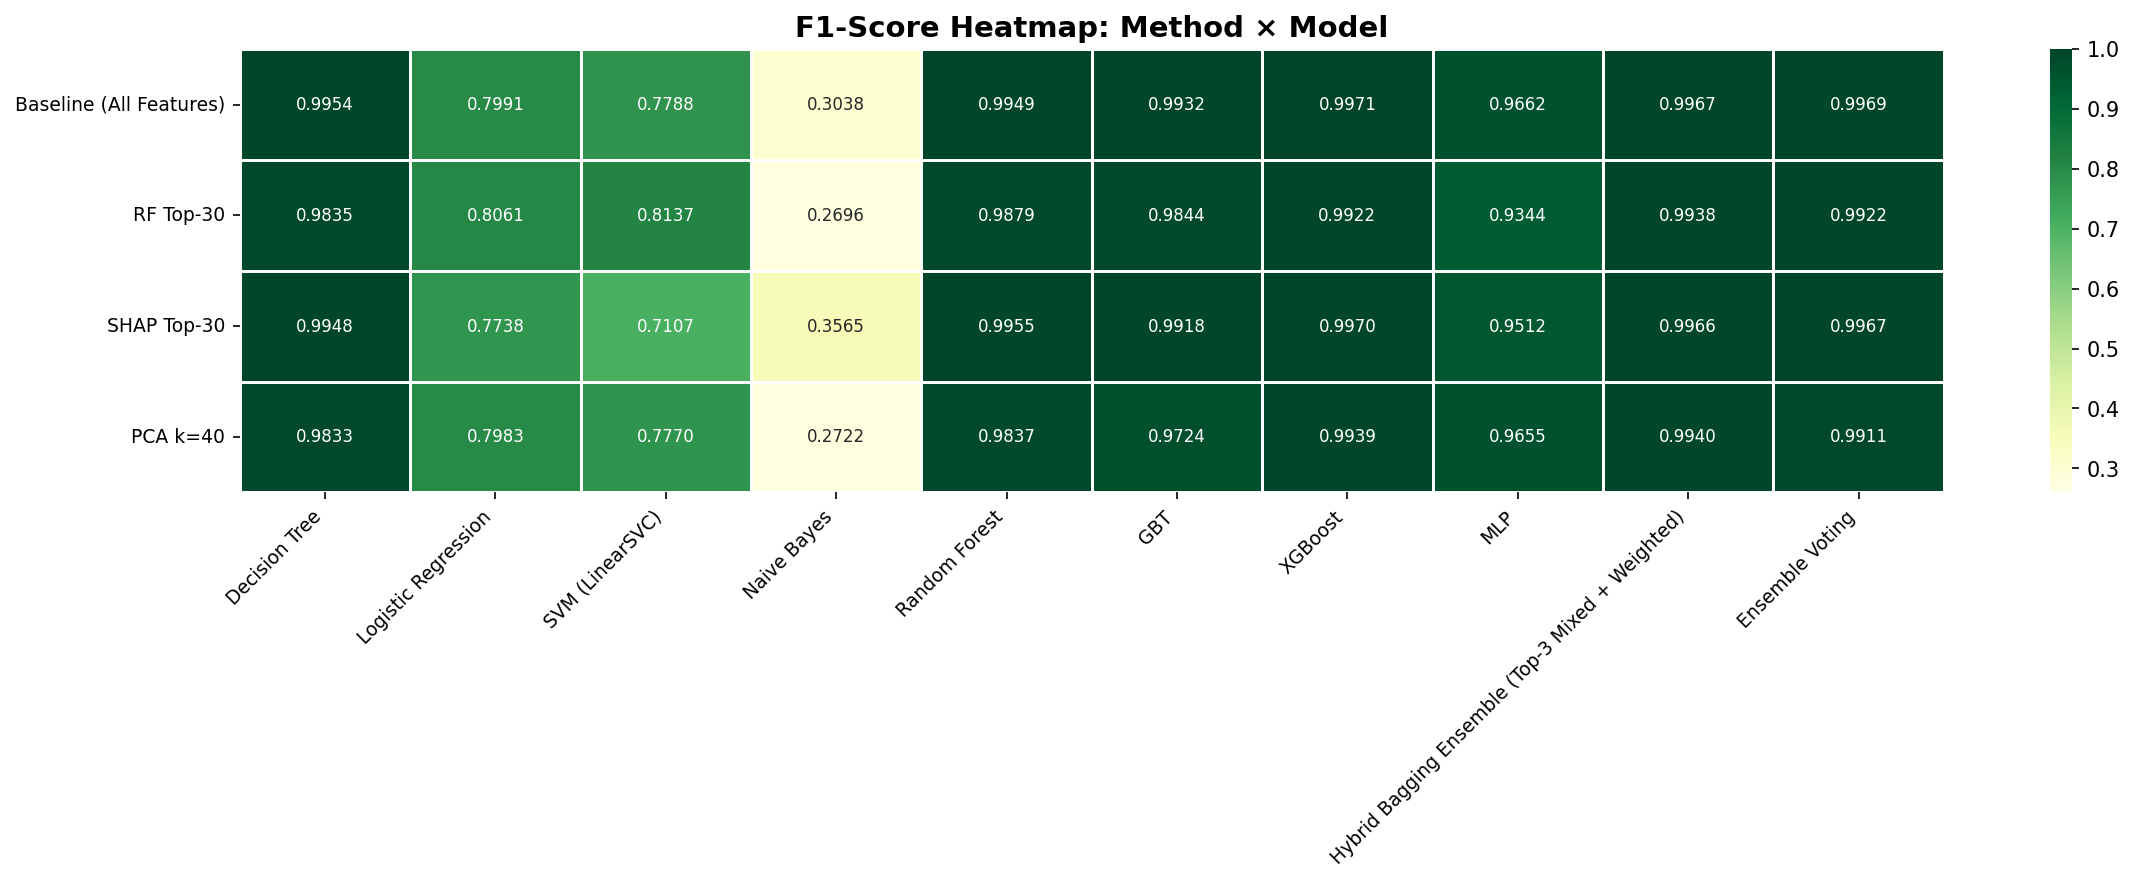
\includegraphics[height=0.74\textheight, width=\textwidth, keepaspectratio]{f1_heatmap.png}}
    {\fbox{\parbox{0.7\textwidth}{\centering\vspace{1.5cm}
      \texttt{f1\_heatmap.png}\vspace{1.5cm}}}}
  \\[0.2em]\footnotesize Nhị phân, đã loại cổng. 8 thuật toán $\times$ 4 phương pháp.
\end{frame}

\begin{frame}{Dự phòng: siêu tham số, cố định từ trước}
  \centering\footnotesize
  \fitwidth{%
  \begin{tabular}{ll}
    \toprule
    Mô hình & Siêu tham số chính \\
    \midrule
    Decision Tree       & maxDepth=15, minInstancesPerNode=5, impurity=entropy \\
    Logistic Regression & maxIter=200, regParam=0.001, L2, threshold=0.5 \\
    SVM (LinearSVC)     & maxIter=200, regParam=0.001 \\
    Naive Bayes         & gaussian, smoothing=1.0 \\
    Random Forest       & numTrees=200, maxDepth=15, featureSubset=sqrt \\
    GBT                 & maxIter=150, maxDepth=6, stepSize=0.05, subsample=0.8 \\
    XGBoost             & n\_estimators=300, max\_depth=8, lr=0.05, subsample=0.8, colsample=0.8 \\
    MLP                 & layers=[$d$,64,32,2], maxIter=150, stepSize=0.01 \\
    \bottomrule
  \end{tabular}
  }
  \\[0.4em]
  \raggedright\scriptsize
  Dùng chung cho mọi phương pháp giảm chiều, nên khác biệt phản ánh
  \emph{phương pháp} chứ không phải việc tinh chỉnh riêng từng mô hình. Trọng số
  lớp cho 6 mô hình, \texttt{scale\_pos\_weight} cho XGBoost; MLP không có trọng
  số (Spark ML không hỗ trợ trọng số mẫu cho nó) --- đã nêu trong phần hạn chế.
  LightGBM bị loại: thư viện gốc qua SynapseML chỉ chạy x86\_64, còn đích triển
  khai là ARM64.
\end{frame}

\begin{frame}{Dự phòng: chi phí huấn luyện và suy luận}
  \centering
  \IfFileExists{../../results/ml_07_cross_method_comparison/train_predict_time.png}
    {\includegraphics[height=0.68\textheight, width=\textwidth, keepaspectratio]{train_predict_time.png}}
    {\fbox{\parbox{0.7\textwidth}{\centering\vspace{1.5cm}
      \texttt{train\_predict\_time.png}\vspace{1.5cm}}}}
  \\[0.2em]\footnotesize
  Đo trên cụm huấn luyện Spark. Độ trễ và thông lượng \emph{trên thiết bị biên}
  thuộc bài hệ thống đi kèm.
\end{frame}

\begin{frame}{Dự phòng: các yếu tố ảnh hưởng tính hợp lệ}
  \begin{itemize}\footnotesize
    \item \textbf{Nội tại.} Xếp hạng RF/SHAP lấy từ tập huấn luyện gốc và giữ
          cố định qua các lần lấy mẫu lại --- nhất quán với thiết kế cố định từ
          trước, nhưng có thể gây rò rỉ nhẹ ở phần xếp hạng. Xếp hạng lại trong
          hai trong sáu lần lấy mẫu chỉ làm F1 lệch $\le 7{,}4\times10^{-5}$,
          và 25--26/30 đặc trưng vẫn được chọn lại. MLP mang hạn chế không có
          trọng số lớp.
    \item \textbf{Ngoại tại.} CICIDS2017 có thể không phản ánh lưu lượng hiện
          tại, và các bộ dữ liệu NIDS chuẩn đều có hạn chế chất lượng đã ghi
          nhận. Kết luận liên bộ dữ liệu dựa trên \emph{mẫu phân tầng} của
          CSE-CIC-IDS2018, chưa phải toàn bộ. Chưa kiểm thử lưu lượng né tránh.
          Bản thân việc khử trùng lặp cũng làm thay đổi phân bố benign/attack.
    \item \textbf{Thống kê.} $N{=}6$ cho kiểm định hoán vị \emph{power} thấp:
          liệt kê đầy đủ hai phía chặn $p$ ở mức $2/2^N$, nên $N{=}6$ \emph{vừa
          đủ} chạm 0,05. Kết luận tương đương không dựa vào $p$ đó mà dựa vào
          TOST, trên cùng sai số Nadeau--Bengio đã tính đến việc các lần lấy
          mẫu chồng nhau. F1 liên bộ không tất định giữa các lượt, nên được báo
          trên 18 lượt. Kiểm định chéo lồng với $N$ lớn hơn là hướng củng cố
          tiếp theo.
  \end{itemize}
\end{frame}

\begin{frame}{Dự phòng: quy kết đặc trưng bằng SHAP}
  \centering
  \IfFileExists{../../results/ml_06_feature_selection_shap/shap_summary_beeswarm.png}
    {\includegraphics[height=0.68\textheight, width=\textwidth, keepaspectratio]{shap_summary_beeswarm.png}}
    {\fbox{\parbox{0.7\textwidth}{\centering\vspace{1.5cm}
      \texttt{shap\_summary\_beeswarm.png}\vspace{1.5cm}}}}
  \\[0.2em]\footnotesize
  SHAP được tính trên \emph{mẫu phân tầng theo lớp} để cả lưu lượng bình thường
  và lưu lượng tấn công đều có mặt trong bảng xếp hạng.
\end{frame}

\end{document}
"
% ---------------------------------------------------------------------
\ifdefined\shownotes
  \usepackage{pgfpages}
  \setbeameroption{show notes on second screen=right}
\fi

\centeredtitles

\graphicspath{%
  {../../results/ml_07_cross_method_comparison/}%
  {../../results/ml_05_shap_explainability/}%
  {../../results/ml_06_feature_selection_shap/}%
  {../../results/ml_09_multiclass_eval/}%
  {../../results/ml_10_leakage_ablation/}%
  {../../results/ml_11_cross_dataset/}%
}

\title{Giảm chiều và chọn lọc đặc trưng cho phát hiện xâm nhập mạng trên Apache Spark ML}
\subtitle{\ldots với quy trình đánh giá loại rò rỉ dữ liệu}
\author{\textbf{Nguyễn Vũ Thái}\inst{1} \and Bùi Văn Dũng\inst{2} \and Đỗ Trí Nhựt\inst{2} \and Nguyễn Văn Dũ\inst{3}}
\institute{\scriptsize
           \inst{1}Phân hiệu tại TP.\ Hồ Chí Minh, Trường Đại học Giao thông Vận tải, TP.\ Hồ Chí Minh, Việt Nam \\
           \inst{2}Trường Đại học Công nghệ Thông tin, ĐHQG-HCM, TP.\ Hồ Chí Minh, Việt Nam \\
           \inst{3}Khoa Công nghệ Thông tin, Trường Đại học Nông Lâm, TP.\ Hồ Chí Minh, Việt Nam}
\date{FAIR'2026}

\begin{document}

% ---------------------------------------------------------------- 0:20
\maketitle
\note{Bảy phút cho một luận điểm duy nhất: trên CICIDS2017, F1 gần như hoàn hảo
thường là tính chất của quy trình đánh giá, không phải của mô hình.}

% ---------------------------------------------------------------- 0:50
% =====================================================================
\section{I.\ VẤN ĐỀ VÀ ĐÓNG GÓP}
% =====================================================================

\begin{frame}{F1 gần như hoàn hảo trên CICIDS2017 là một dấu hiệu đáng ngờ}
  \begin{columns}[T]
    \begin{column}{0.55\textwidth}
      \textbf{Hai vấn đề, thường được xét riêng}
      \begin{itemize}
        \item \key{Chi phí.} $\approx$80 đặc trưng mỗi luồng.
        \item \key{Độ tin cậy.} F1 nhị phân gần hoàn hảo thường báo hiệu
              \bad{rò rỉ dữ liệu}.
      \end{itemize}
      \vspace{0.5em}
      \textbf{Hai nguồn rò rỉ cụ thể}
      \begin{enumerate}
        \item \texttt{destination\_port} mã hóa \emph{dịch vụ bị tấn công}.
        \item \bad{Trùng lặp ở mức đặc trưng} sống sót qua khử trùng lặp
              toàn dòng --- cùng một mẫu nằm ở \emph{cả} tập huấn luyện
              \emph{và} tập kiểm tra.
      \end{enumerate}
    \end{column}
    \begin{column}{0.42\textwidth}
      \begin{alertblock}{Bài báo này}
        So sánh bốn chiến lược giảm chiều trên cùng tám bộ phân loại Spark ML
        --- nhưng trước hết làm cho \emph{quy trình đánh giá} đáng tin đã.
      \end{alertblock}
      \begin{exampleblock}{Đóng góp nằm ở giao thức đo}
        Không phải ``phương pháp nào thắng'' mà là \key{đo thế nào để câu trả
        lời có ý nghĩa}.
      \end{exampleblock}%
    \end{column}
  \end{columns}
  \note{Rò rỉ dữ liệu: thông tin không có lúc triển khai lọt vào huấn luyện hoặc
  đánh giá. Định vị bài báo là bài về phép đo. Cổng đích cho mô hình một đường tắt
  từ cổng sang nhãn; 80 đặc trưng thì tốn cả khi huấn luyện, khi suy luận và
  khi nhồi lên thiết bị biên. Cả hai nguồn rò rỉ đều được loại trước khi chia
  tập.}
\end{frame}

% ---------------------------------------------------------------- 0:35
\begin{frame}{Các đóng góp}
  \begin{enumerate}
    \item \key{So sánh thống nhất} giữa RF Importance, SHAP và PCA trên cùng 8
          thuật toán Spark ML $+$ 2 mô hình tổ hợp, trên CICIDS2017.
    \item SHAP được đặt \key{trực tiếp} cạnh RF Importance trên cùng tập huấn
          luyện.
    \item Quy trình \key{loại rò rỉ và có kiểm định thống kê}: loại đặc trưng rò
          rỉ, khử trùng lặp ở mức đặc trưng một cách tất định, chọn mô hình trên
          tập kiểm định, kiểm định hoán vị ghép cặp liệt kê đầy đủ kèm hiệu chỉnh
          Nadeau--Bengio.
    \item \key{Đánh giá đa lớp theo từng loại tấn công} --- nơi các phương pháp
          thực sự khác nhau.
    \item Khuyến nghị \key{có tính tới thiết bị biên}: F1 \emph{và} số đặc trưng
          \emph{và} kích thước mô hình, cho Jetson Orin Nano Super (phần triển
          khai nằm ở một bài hệ thống đi kèm).
  \end{enumerate}
  \note{Năm đóng góp; ba, bốn và năm là những thứ ít khi được làm cùng nhau.}
\end{frame}

% ---------------------------------------------------------------- 0:55
% =====================================================================
\section{II.\ QUY TRÌNH LOẠI RÒ RỈ}
% =====================================================================

\begin{frame}{Quy trình loại rò rỉ}
  \begin{columns}[c]
    \begin{column}{0.5\textwidth}
      \centering
      \resizebox{0.98\textwidth}{!}{%
      \begin{tikzpicture}[
        font=\footnotesize, node distance=2.6mm, >=Stealth,
        box/.style={draw=gray!60, rounded corners=2pt, align=center, inner sep=4pt, minimum width=7.6cm},
        hl/.style={box, draw=accRed, fill=accRed!10},
        ed/.style={box, draw=accGreen!80!black, fill=accGreen!10},
        arr/.style={-{Stealth[length=2mm]}, semithick}]
        \node[box] (raw)  {CICIDS2017 --- 8 tệp CSV, $\approx$2,8 triệu luồng};
        \node[hl, below=of raw] (prep) {\textbf{Chuẩn bị dữ liệu loại rò rỉ}\\
              loại \texttt{destination\_port} $\cdot$ khử trùng lặp mức đặc trưng};
        \node[box, below=of prep] (split) {Chia 80/20 (hạt giống cố định) $\cdot$ Parquet};
        \node[box, below=of split] (strat) {\textbf{4 chiến lược}: Cơ sở $|$ RF Top-$K$ $|$ SHAP Top-$K$ $|$ PCA\\
              (xếp hạng khớp \emph{chỉ trên tập huấn luyện})};
        \node[box, below=of strat] (clf) {8 bộ phân loại Spark ML $+$ 2 tổ hợp};
        \node[hl, below=of clf] (val) {Chọn mô hình trên tập kiểm định $\cdot$ kiểm định hoán vị ghép cặp\\
              khoảng tin cậy Nadeau--Bengio $\cdot$ cỡ hiệu ứng $\cdot$ đa lớp};
        \node[ed, below=of val] (edge) {SHAP Top-30 $\rightarrow$ Jetson Orin Nano Super};
        \draw[arr] (raw)--(prep); \draw[arr] (prep)--(split); \draw[arr] (split)--(strat);
        \draw[arr] (strat)--(clf); \draw[arr] (clf)--(val); \draw[arr] (val)--(edge);
      \end{tikzpicture}}
    \end{column}
    \begin{column}{0.47\textwidth}
      \textbf{Mỗi bước chặn một đường rò rỉ}
      \begin{itemize}\footnotesize
        \item Loại cổng đích: chặn \bad{đường tắt cổng $\to$ nhãn}.
        \item Khử trùng lặp \emph{trước} khi chia: không mẫu nào ở cả hai tập.
        \item Scaler, PCA, xếp hạng RF/SHAP chỉ \emph{fit} trên tập huấn luyện.
        \item Chọn mô hình trên tập kiểm định (20\% tập huấn luyện): tập kiểm
              tra \bad{không} tham gia bước chọn nào.
      \end{itemize}
      \vspace{0.2em}
      \textbf{Thiết kế cố định \emph{từ trước}}
      \begin{itemize}\footnotesize
        \item Quét $K \in \{20,30,40\}$ tách khỏi pha xác nhận 4 cấu hình:
              Cơ sở, RF Top-30, SHAP Top-30, PCA $k{=}40$.
      \end{itemize}
    \end{column}
  \end{columns}
  \note{Đi từ trên xuống, mỗi khối đỏ là một chỗ rò rỉ bị chặn. Không cấu hình
  nào được chọn theo F1 trên tập kiểm tra. Siêu tham số dùng chung cho mọi
  phương pháp, nên khác biệt phản ánh phương pháp chứ không phải việc tinh
  chỉnh.}
\end{frame}

% ---------------------------------------------------------------- 1:05
\begin{frame}{Khử trùng lặp tất định và thiết lập thực nghiệm}
  \begin{columns}[T]
    \begin{column}{0.52\textwidth}
      \textbf{Chuẩn bị dữ liệu, trước khi chia tập}
      \begin{enumerate}\footnotesize
        \item Gộp 8 tệp CSV; $\pm\infty \to$ NaN; bỏ dòng thiếu, dòng trùng.
        \item Nhãn: BENIGN $\to 0$, mọi tấn công $\to 1$.
        \item Đặc trưng $\mathcal{F}$: cột số, \emph{trừ} cổng, giao thức,
              định danh.
        \item Nhóm dòng giống hệt nhau trên $\mathcal{F}$:
              mâu thuẫn nhãn $\to$ \bad{loại cả nhóm}
              (\num{270 nhóm, 44.260 dòng}); còn lại $\to$ giữ \emph{một}
              đại diện tất định.
        \item Chia 80/20, hạt giống cố định.
      \end{enumerate}
    \end{column}
    \begin{column}{0.45\textwidth}
      \centering\scriptsize
      \fitwidth{%
      \begin{tabular}{lr}
        \toprule
        \multicolumn{2}{l}{\textbf{CICIDS2017} (sau xử lý)} \\
        \midrule
        Đặc trưng số             & 77 \\
        Huấn luyện / kiểm tra    & 1.785.349 / 447.275 \\
        Tổng                     & 2.232.624 \\
        \midrule
        \multicolumn{2}{l}{\textbf{CSE-CIC-IDS2018} (mẫu phân tầng 20\%)} \\
        \midrule
        Trước / sau khử trùng lặp & $\sim$3,14 / $\sim$2,39 triệu \\
        \bottomrule
      \end{tabular}
      }
      \vspace{0.4em}

      \raggedright
      \begin{itemize}\scriptsize
        \item \textbf{Hạ tầng:} Spark 3.4.1; 2$\times$ Jetson Orin Nano Super
              (8\,GB) làm worker, máy chủ \emph{chỉ} làm master.
        \item \textbf{Chỉ số:} ưu tiên \key{AUC-PR} và \key{recall tấn công}
              hơn accuracy vì dữ liệu mất cân bằng.
        \item Mã nguồn công khai; chạy lại được trên một máy.
      \end{itemize}
    \end{column}
  \end{columns}
  \note{Chỗ nhiều người làm sai là nhóm mâu thuẫn nhãn: giữ ngẫu nhiên một dòng
  thì nhãn phụ thuộc cách Spark chia phân vùng, mỗi lần chạy ra một bộ dữ liệu
  khác; loại cả nhóm thì kết quả tất định. Lỗi nhãn này của CICIDS2017 đã được
  Lanvin et al.\ ghi nhận. Cột bị loại cụ thể là destination\_port,
  source\_port, protocol và các cột định danh. Thời gian huấn luyện ở các slide
  sau là thời gian trên hai Jetson, không phải trên máy chủ.}
\end{frame}

% ---------------------------------------------------------------- 1:00
% =====================================================================
\section{III.\ KẾT QUẢ VÀ KẾT LUẬN}
% =====================================================================

\begin{frame}{Kết quả 1: bỏ được 60\% đặc trưng}
  \begin{columns}[T]
    \begin{column}{0.55\textwidth}
      \centering\small
      \fitwidth{%
      \begin{tabular}{llccc}
        \toprule
        Phương pháp & Mô hình & F1 & Huấn luyện (s) & Đ.trưng \\
        \midrule
        Cơ sở                & XGBoost & 0,9971 & 4615,5 & 77 \\
        \textbf{SHAP Top-30} & XGBoost & \num{0,9970} & \num{1226,1} & \num{30} \\
        PCA $k{=}40$         & XGBoost & 0,9939 & 1444,8 & 40 \\
        RF Top-30            & XGBoost & 0,9922 & 1295,1 & 30 \\
        \bottomrule
      \end{tabular}
      }
      \par{\scriptsize Huấn luyện (s): cụm Spark gồm 2$\times$ Jetson Orin Nano
      Super; máy chủ chỉ làm master, không chạy executor.}
      \vspace{0.5em}

      \footnotesize
      \fitwidth{%
      \begin{tabular}{lccc}
        \toprule
        Thuật toán & RF Top-30 & SHAP Top-30 & $\Delta$ \\
        \midrule
        Random Forest & 0,9879 & 0,9955 & \good{$+$0,77\%} \\
        XGBoost       & 0,9922 & 0,9970 & \good{$+$0,48\%} \\
        GBT           & 0,9844 & 0,9918 & \good{$+$0,75\%} \\
        Decision Tree & 0,9835 & 0,9948 & \good{$+$1,15\%} \\
        \bottomrule
      \end{tabular}
      }
    \end{column}
    \begin{column}{0.43\textwidth}
      \begin{itemize}\small
        \item SHAP Top-30 giữ được F1 của cấu hình cơ sở trong khi cắt
              \good{$\approx$60\% đặc trưng} và \good{$\approx$73\% thời gian
              huấn luyện}.
        \item Ở \emph{cùng} số đặc trưng, SHAP thắng RF Importance trên mọi
              thuật toán dạng cây.
        \item PCA dùng $k{=}40$ vì nó \emph{trích xuất} chứ không
              \emph{chọn lọc} --- mỗi thành phần chỉ mang một phần phương sai.
              Rẻ hơn cấu hình cơ sở, nhưng không giải thích được.
      \end{itemize}
    \end{column}
  \end{columns}
  \note{Hai bảng, một thông điệp: SHAP Top-30 là điểm vận hành. Cùng độ chính
  xác, ít hơn 60 phần trăm đặc trưng, và giải thích được — điều quan trọng với
  phân tích viên SOC và với thiết bị biên ở phía sau.}
\end{frame}

% ---------------------------------------------------------------- 0:55
\begin{frame}{Kết quả 2: cổng đích rò rỉ bao nhiêu tùy họ mô hình}
  \begin{columns}[T]
    \begin{column}{0.50\textwidth}
      \centering\footnotesize
      \fitwidth{%
      \begin{tabular}{lccc}
        \toprule
        Thuật toán & F1 (loại cổng) & F1 (giữ cổng) & $\Delta$F1 \\
        \midrule
        SVM (LinearSVC)     & 0,7859 & 0,8274 & \bad{$+$0,0415} \\
        Logistic Regression & 0,7986 & 0,8381 & \bad{$+$0,0395} \\
        Naive Bayes         & 0,2985 & 0,3093 & $+$0,0108 \\
        MLP                 & 0,9660 & 0,9711 & $+$0,0052 \\
        GBT                 & 0,9924 & 0,9941 & $+$0,0017 \\
        Decision Tree       & 0,9953 & 0,9966 & $+$0,0014 \\
        Random Forest       & 0,9954 & 0,9964 & $+$0,0010 \\
        XGBoost             & 0,9972 & 0,9979 & $+$0,0007 \\
        \bottomrule
      \end{tabular}
      }
      \\[0.3em]
      \scriptsize Hai lượt trên \emph{cùng} một phép chia, chỉ khác giữ hay
      loại \texttt{destination\_port}; bài toán nhị phân.
    \end{column}
    \begin{column}{0.47\textwidth}
      \begin{itemize}\footnotesize
        \item \textbf{Họ cây} chỉ được lợi $+$0,0007 đến $+$0,0017: chúng dựng
              lại cùng biên quyết định từ thống kê hành vi của luồng.
        \item \textbf{Mô hình tuyến tính} được lợi tới \bad{$+$0,04}, gấp
              khoảng 40 lần: chúng bám vào cổng như một định danh dịch vụ.
        \item Random Forest: F1 0,9964 $\to$ 0,9954, recall tấn công
              0,9988 $\to$ 0,9961. Chiều hướng vẫn nhất quán với rò rỉ.
        \item Tác vụ nhị phân trong-miền đã gần bão hòa sau khử trùng lặp, nên
              mức chênh ở họ cây nhỏ.
      \end{itemize}
    \end{column}
  \end{columns}
  \takeaway{Ablation trên \emph{một} mô hình \key{không giới hạn được} mức rò rỉ
  của một lớp mô hình khác. Mọi kết quả sau đều dùng cấu hình đã loại cổng.}
  \note{Bài bản nộp chỉ đo trên Random Forest; bản camera-ready chạy cả tám thuật
  toán theo góp ý phản biện. Con số 0,001 là đặc tính của họ cây, không phải của
  bộ dữ liệu.}
\end{frame}

% ---------------------------------------------------------------- 1:00
\begin{frame}{Kết quả 3: kiểm định sự khác biệt, rồi kiểm định sự tương đương}
  \begin{columns}[T]
    \begin{column}{0.47\textwidth}
      \centering\footnotesize
      \fitwidth{%
      \begin{tabular}{llc}
        \toprule
        Phương pháp & Mô hình & F1 (TB $\pm$ CI95) \\
        \midrule
        Cơ sở       & XGBoost & 0,99734 $\pm$ 0,00007 \\
        SHAP Top-30 & XGBoost & 0,99720 $\pm$ 0,00009 \\
        \midrule
        \multicolumn{3}{c}{\footnotesize hoán vị ghép cặp $p = 0{,}031$;\ $d \approx 1{,}94$} \\
        \bottomrule
      \end{tabular}
      }
      \vspace{0.4em}

      \fitwidth{%
      \begin{tabular}{lc}
        \toprule
        \multicolumn{2}{l}{\textbf{TOST} (hai kiểm định một phía)} \\
        \midrule
        Biên tương đương, khai báo trước & $\pm$0,001 F1 \\
        Sai số dùng để kiểm định         & Nadeau--Bengio \\
        $p_{\text{TOST}}$                & \good{$3{,}9\times10^{-6}$} \\
        Biên nhỏ nhất chứng minh được ($\alpha{=}0{,}05$) & \good{$\pm2{,}3\times10^{-4}$} \\
        \bottomrule
      \end{tabular}
      }
    \end{column}
    \begin{column}{0.50\textwidth}
      \begin{itemize}\footnotesize
        \item $N{=}6$ lần \emph{lấy mẫu lại} ghép cặp: phương sai phản ánh
              việc lấy mẫu dữ liệu, không chỉ hạt giống.
        \item Hoán vị hai phía, \key{liệt kê đủ} $2^6$ tổ hợp dấu: $p$ nhỏ
              nhất là $2/2^6$, nên $N \geq 6$ là \emph{bắt buộc}.
        \item Lấy mẫu chồng nhau phá vỡ tính độc lập của $t$ $\rightarrow$
              dùng CI \key{hiệu chỉnh Nadeau--Bengio}.
        \item $p = 0{,}031$ nằm ngay sàn phân giải, trong khi cách biệt chỉ
              $\approx$0,0001. Kiểm định ý nghĩa \bad{không} chứng minh được
              tương đương, nên bài báo kiểm định tương đương \emph{trực tiếp}
              bằng TOST.
      \end{itemize}
    \end{column}
  \end{columns}
  \takeaway{Cơ sở và SHAP Top-30 \key{tương đương theo nghĩa khẳng định}: chênh
  lệch thật nhỏ hơn $2{,}3\times10^{-4}$ F1. Tính giải thích được và chi phí mới
  quyết định lựa chọn.}
  \note{Hai bước: kiểm định hoán vị cho thấy khác biệt rất nhỏ nhưng có ý
  nghĩa ở sát sàn, rồi TOST cho thấy khác biệt đó nằm gọn trong biên 0,001 khai
  báo từ trước. Nói "tương đương" là có kiểm định, không phải suy từ một p lớn.}
\end{frame}

% ---------------------------------------------------------------- 0:55
\begin{frame}{Kết quả 4: F1 nhị phân che giấu các lớp hiếm}
  \begin{columns}[c]
    \begin{column}{0.40\textwidth}
      \centering
      \IfFileExists{../../results/ml_09_multiclass_eval/confusion_matrix.png}
        {\includegraphics[width=0.98\textwidth]{confusion_matrix.png}}
        {\fbox{\parbox{0.8\textwidth}{\centering\vspace{1.2cm}
          \texttt{confusion\_matrix.png}\vspace{1.2cm}}}}
    \end{column}
    \begin{column}{0.58\textwidth}
      \centering\footnotesize
      \fitwidth{%
      \begin{tabular}{lccc}
        \toprule
        Lớp & Số mẫu & Recall & F1 \\
        \midrule
        Benign                & 380.119 & 0,9997 & 0,9989 \\
        DoS Hulk              & 34.446  & 0,9904 & 0,9947 \\
        Web -- Brute Force    & 311     & 0,7299 & 0,7323 \\
        Bot                   & 290     & \bad{0,4552} & 0,6256 \\
        Web -- XSS            & 111     & \bad{0,0270} & 0,0526 \\
        Web -- SQL Injection  & 6       & \bad{0,0000} & 0,0000 \\
        \midrule
        \multicolumn{2}{l}{weighted-F1 $=$ 0,998} &
        \multicolumn{2}{l}{\bad{macro-F1 $=$ 0,806}} \\
        \bottomrule
      \end{tabular}
      }
      \par\vspace{0.2em}
      \raggedright\scriptsize
      Hai kiểu sai, theo \emph{nơi lỗi rơi vào}:
      \begin{itemize}\scriptsize
        \item \textbf{Nhầm loại nhưng vẫn bắt}: 81/111 XSS rơi vào Web Brute
              Force --- \good{76\% vẫn bị gắn cờ} ở mức nhị phân.
        \item \textbf{Lọt vào Benign} (nguy hiểm): cả 6 SQL Injection,
              \bad{54\% Bot} (158/290), 27\% Brute Force.
      \end{itemize}
    \end{column}
  \end{columns}
  \note{Weighted F1 0,998 so với macro F1 0,806. Ba nguyên nhân: mất cân bằng
  cực độ, 6--311 mẫu so với 380 nghìn Benign; không còn đường tắt cổng 80 thì
  luồng HTTP ngắn của tấn công web trông như lướt web thường; beaconing của Bot
  C\&C giống lưu lượng nền khi mất định danh dịch vụ. Recall 0,027 của XSS ở đây thay
  cho một con số từng bị rò rỉ thổi phồng. Hai lớp không có trên bảng: PortScan
  F1 0,976 và Infiltration F1 0,800 (12 mẫu). Bảy lớp còn lại, gồm cả
  Heartbleed, đều đạt F1 từ 0,95 trở lên.}
\end{frame}

% ---------------------------------------------------------------- 1:10
\begin{frame}{Kết quả 5: điểm số không sống sót khi đổi testbed}
  \begin{columns}[T]
    \begin{column}{0.47\textwidth}
      \centering\footnotesize
      \fitwidth{%
      \begin{tabular}{lcc}
        \toprule
        Huấn luyện $\to$ Kiểm tra & F1 & AUC-PR \\
        \midrule
        2017 $\to$ 2017 (trong-miền)  & \good{0,9953} & \good{0,9997} \\
        2017 $\to$ 2018 (11 lượt)     & \bad{0,029--0,085} & \bad{0,4778} \\
        2017 $\to$ 2018 (7 lượt)      & \bad{0,185--0,301} & \bad{0,4960} \\
        2018 $\to$ 2018 (trong-miền)  & \good{0,9246} & \good{0,9679} \\
        2018 $\to$ 2017               & \bad{0,0544} \tiny$\pm$0,0019 & \bad{0,1926} \\
        \bottomrule
      \end{tabular}
      }
      \\[0.3em]
      \scriptsize\raggedright
      18 lượt cùng mã nguồn và dữ liệu (13 hạt giống, 5 hạt giống chạy hai
      lần). 2017 = CICIDS2017, 2018 = CSE-CIC-IDS2018.
    \end{column}
    \begin{column}{0.50\textwidth}
      \begin{itemize}\scriptsize
        \item AUC-PR sụp \bad{0,9997 $\to$ 0,4849} (trung bình 18 lượt) và
              \bad{0,9679 $\to$ 0,1926}. Recall 0,073 / 0,030, precision
              0,772 / 0,272: mô hình \key{bỏ sót} tấn công của testbed kia.
        \item 2017$\to$2018: F1 có \key{hai chế độ rời nhau}. Trung bình
              0,1276 rơi vào khoảng trống; CI95 của nó chỉ chứa 1/18 lượt.
        \item 5 hạt giống chạy lại: 2 đổi chế độ. Quá trình fit phân tán
              quyết định, không phải hạt giống.
        \item AUC-PR hai chế độ như nhau (Welch $|t|{=}1{,}3$): chỉ ngưỡng 0,5
              cắt qua một cụm luồng gần giống nhau, cả cụm lật cùng lúc.
      \end{itemize}
    \end{column}
  \end{columns}
  \takeaway{F1 liên bộ của \emph{một} lượt chỉ cho biết lượt đó rơi vào chế độ
  nào. Bài báo báo cáo cả phân bố và so sánh bằng \key{AUC-PR}.}
  \note{Nguyên nhân dịch chuyển: khác phiên bản CICFlowMeter nên thang đo đặc
  trưng đổi, khác cấu hình mạng, khác công cụ tấn công (HOIC/LOIC-HTTP chỉ có ở
  2018). Trong 5 hạt giống chạy hai lần, 3 giữ nguyên chế độ và 2 đổi chế độ.
  Không làm nhẹ con số này. Bản nộp ban đầu báo một con số F1 duy nhất;
  lặp lại thí nghiệm cho thấy con số đó không tái lập được giữa các lượt, nên
  bản camera-ready báo hai chế độ. Kết luận không đổi, thậm chí chắc hơn: lượt
  tốt nhất trong 18 lượt cũng chỉ đạt F1 0,30 so với 0,9953 trong-miền.}
\end{frame}

% ---------------------------------------------------------------- 1:00
\begin{frame}{Kết quả 6: thích ứng miền --- cái gì cứu được, cái gì không}
  \begin{columns}[T]
    \begin{column}{0.53\textwidth}
      \centering\footnotesize
      \fitwidth{%
      \begin{tabular}{lccc}
        \toprule
        Cách thích ứng & Nhãn đích & 2017$\to$2018 & 2018$\to$2017 \\
        \midrule
        Không thích ứng                  & không & 0,029--0,301 & 0,054 \\
        Refit scaler trên miền đích      & không & \bad{0,000} & \bad{0,000} \\
        CORAL                            & không & \bad{0,000} & \bad{0,000} \\
        \midrule
        Chỉ 1\% dữ liệu đích             & có    & \good{0,922} & \good{0,990} \\
        Nguồn 1,79 triệu $+$ 1\% đích    & có    & 0,803 & 0,961 \\
        \bottomrule
      \end{tabular}
      }
      \\[0.3em]
      \scriptsize\raggedright
      Giá trị là F1. 1\% tập huấn luyện của miền đích $\approx$19 nghìn luồng
      (18 nghìn cho chiều ngược lại). Mỗi cách thích ứng được so với lượt không
      thích ứng của chính nó.
    \end{column}
    \begin{column}{0.44\textwidth}
      \begin{itemize}\scriptsize
        \setlength{\itemsep}{0.25em}
        \item Refit scaler và CORAL, không nhãn và không huấn luyện lại, đưa F1
              về \bad{0} ở cả hai chiều, trong cả 3 lượt. Dịch chuyển nằm ở
              phân phối có điều kiện, không chỉ ở trung bình và hiệp phương sai.
        \item CORAL vẫn nâng AUC-PR chiều 2018$\to$2017 (0,179 $\to$ 0,250)
              dù F1 bằng 0: thứ hạng tốt lên, nhưng ngưỡng 0,5 fit trên miền
              nguồn không còn đúng. Thích ứng phải hiệu chỉnh cả ngưỡng.
        \item Gán nhãn một ít dữ liệu mạng mới hiệu quả ngay. Gộp thêm dữ liệu
              nguồn lại \bad{kém hơn} bỏ hẳn nó.
      \end{itemize}
    \end{column}
  \end{columns}
  \takeaway{Thích ứng miền là \key{điều kiện tiên quyết} để chuyển giao, và cách
  rẻ nhất ở đây là gán nhãn một ít lưu lượng của chính mạng đích.}
  {\tiny\textcolor{gray!55!black}{Sun, Feng \& Saenko, \emph{Return of
  frustratingly easy domain adaptation}, AAAI 2016.}}
  \note{Hai baseline không giám sát được thêm theo góp ý phản biện, và cả hai
  đều thất bại về F1. Bài học không phải là thích ứng vô ích, mà là nắn lại
  thang đo đặc trưng thôi thì chưa đủ.}
\end{frame}

% ---------------------------------------------------------------- 0:40
\begin{frame}{Kết luận}
  \begin{columns}[T]
    \begin{column}{0.52\textwidth}
      \textbf{Những gì đã chỉ ra}
      \begin{itemize}\footnotesize
        \item SHAP Top-30: \good{$\approx$60\% ít đặc trưng}, $\approx$73\% ít
              thời gian huấn luyện.
        \item Cơ sở và SHAP Top-30 \key{tương đương} trong
              $\pm2{,}3\times10^{-4}$ F1 (TOST).
        \item Rò rỉ cổng: $+$0,001 với cây, \bad{$+$0,04} với mô hình tuyến tính.
        \item \bad{macro-F1 0,806} so với weighted-F1 0,998.
        \item AUC-PR liên bộ \bad{0,48 / 0,19}; F1 liên bộ có hai chế độ.
        \item Scaler, CORAL: F1 bằng 0; 1\% nhãn đích: \good{0,92 / 0,99}.
      \end{itemize}
    \end{column}
    \begin{column}{0.45\textwidth}
      \textbf{Đóng góp}
      \begin{itemize}\footnotesize
        \item \key{Đo thế nào cho đáng tin}, quan trọng ngang với phương pháp
              nào thắng.
      \end{itemize}
      \textbf{Hướng tiếp theo}
      \begin{itemize}\footnotesize
        \item Ablation chính bước khử trùng lặp.
        \item Toàn bộ CSE-CIC-IDS2018; RoEduNet, CIC-IoT.
        \item Tập SHAP Top-30 có chuyển được sang bộ khác?
        \item Tăng $N$ bằng kiểm định chéo lồng.
      \end{itemize}
    \end{column}
  \end{columns}
  \vfill
  \centering \key{Xin cảm ơn --- kính mời câu hỏi}
  \note{Kết bằng giao thức đo, không kết bằng bảng xếp hạng.}
\end{frame}

% ---------------------------------------------------------------- 7:00
\begin{frame}{Tài liệu tham khảo chính}
  \begin{itemize}\scriptsize
    \setlength{\itemsep}{0.1em}
    \item[{[1]}] Sharafaldin, I., Lashkari, A.\,H. \& Ghorbani, A.\,A.
          \emph{Toward generating a new intrusion detection dataset and
          intrusion traffic characterization}. ICISSP 2018.
          \hfill{\key{CICIDS2017}}
    \item[{[2]}] Lanvin, M. et al. \emph{Errors in the CICIDS2017 Dataset and the
          Significant Differences in Detection Performances It Makes}.
          CRiSIS 2022.
          \hfill{\key{mâu thuẫn nhãn}}
    \item[{[3]}] Arp, D. et al. \emph{Dos and Don'ts of Machine Learning in Computer
          Security}. USENIX Security 2022.
          \hfill{\key{bẫy rò rỉ}}
    \item[{[4]}] Lundberg, S.\,M. \& Lee, S.-I. \emph{A unified approach to
          interpreting model predictions}. NeurIPS 2017.
          \hfill{\key{SHAP}}
    \item[{[5]}] Nadeau, C. \& Bengio, Y. \emph{Inference for the Generalization
          Error}. Machine Learning 52(3), 2003.
          \hfill{\key{CI hiệu chỉnh}}
    \item[{[6]}] D'hooge, L. et al. \emph{Inter-dataset generalization strength of
          supervised machine learning methods for intrusion detection}.
          J.\ Information Security and Applications 54, 2020.
          \hfill{\key{liên bộ dữ liệu}}
    \item[{[7]}] Zaharia, M. et al. \emph{Spark: Cluster computing with working
          sets}. HotCloud 2010.
          \hfill{\key{Spark ML}}
    \item[{[8]}] CIC \& CSE. \emph{CSE-CIC-IDS2018 dataset}. 2018.
          \hfill{\key{đích liên bộ dữ liệu}}
    \item[{[9]}] Schuirmann, D.\,J. \emph{A comparison of the two one-sided tests
          procedure and the power approach for assessing the equivalence of
          average bioavailability}. J.\ Pharmacokinetics and
          Biopharmaceutics 15(6), 1987.
          \hfill{\key{TOST}}
    \item[{[10]}] Sun, B., Feng, J. \& Saenko, K. \emph{Return of frustratingly
          easy domain adaptation}. AAAI 2016.
          \hfill{\key{CORAL}}
  \end{itemize}
  \note{Không trình bày --- để trên màn hình trong lúc nhận câu hỏi, nên nguồn
  luôn hiện sẵn nếu khán giả hỏi. Danh sách đầy đủ nằm trong bài báo.}
\end{frame}

% =====================================================================
\appendix

\begin{frame}[standout]
  Slide dự phòng
\end{frame}

\begin{frame}{Dự phòng: bản đồ nhiệt F1, phương pháp $\times$ thuật toán}
  \centering
  \IfFileExists{../../results/ml_07_cross_method_comparison/f1_heatmap.png}
    {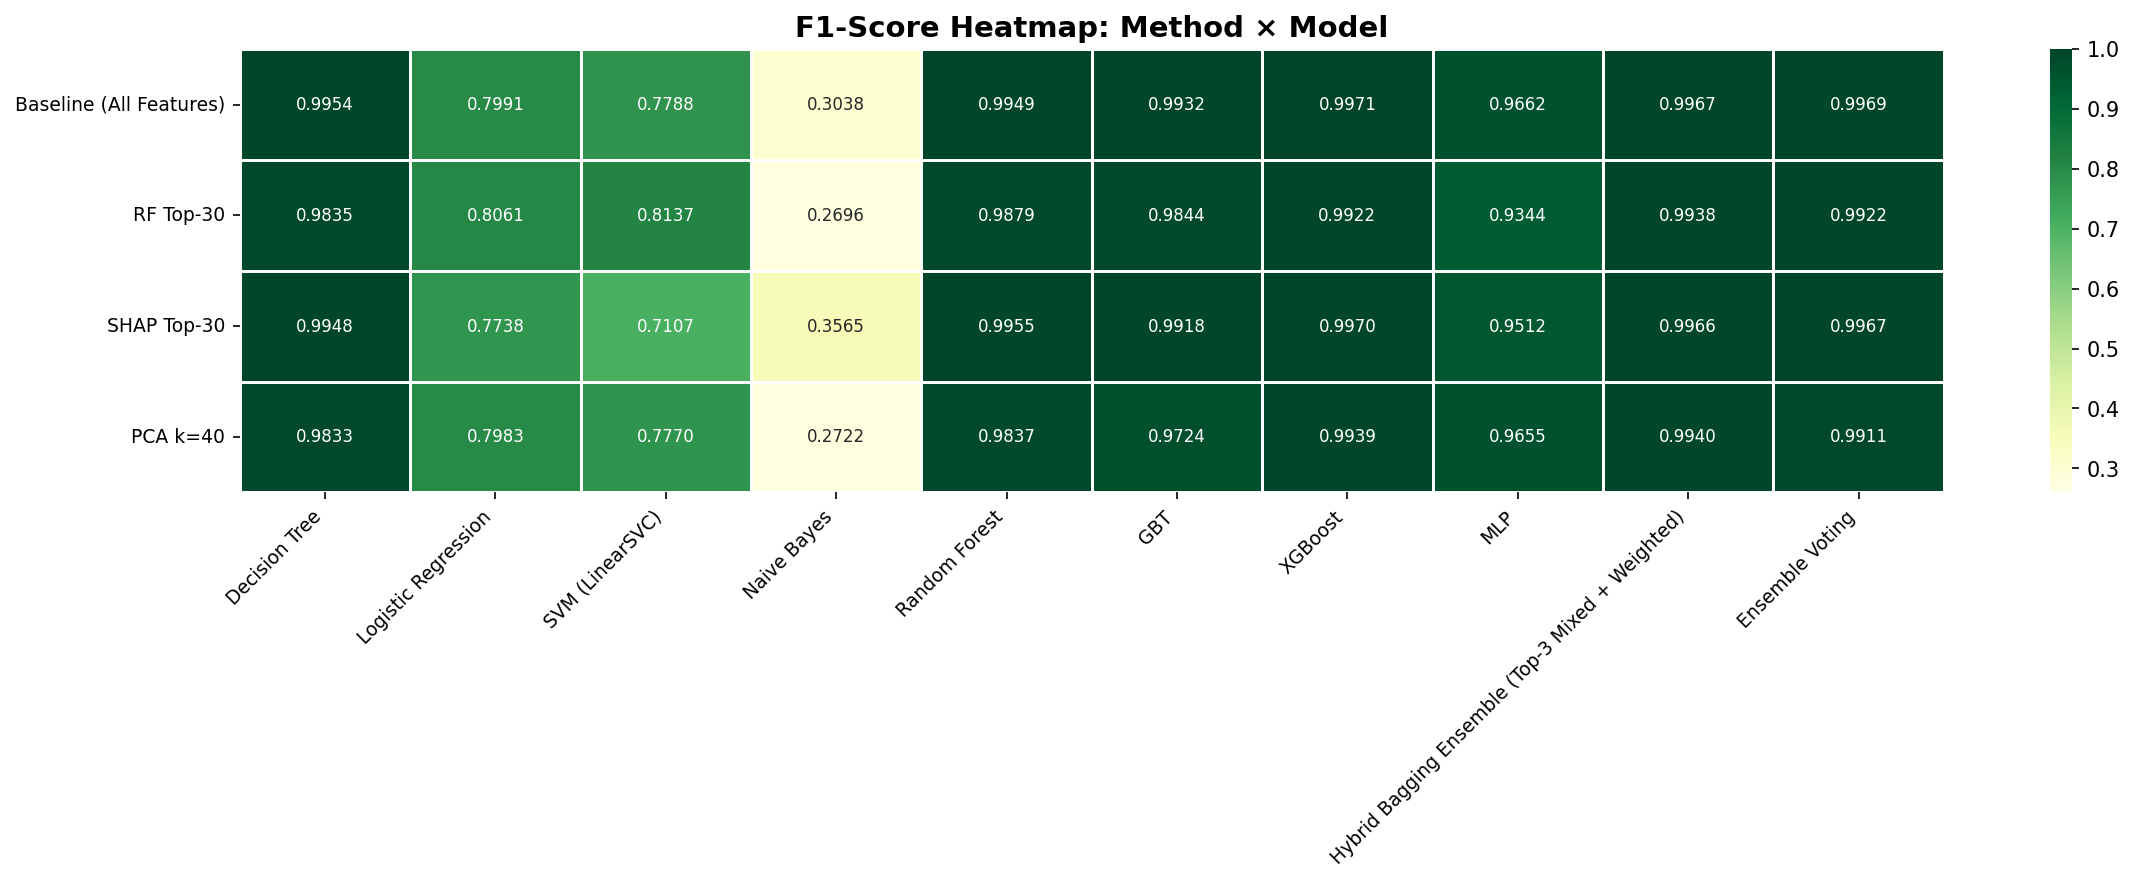
\includegraphics[height=0.74\textheight, width=\textwidth, keepaspectratio]{f1_heatmap.png}}
    {\fbox{\parbox{0.7\textwidth}{\centering\vspace{1.5cm}
      \texttt{f1\_heatmap.png}\vspace{1.5cm}}}}
  \\[0.2em]\footnotesize Nhị phân, đã loại cổng. 8 thuật toán $\times$ 4 phương pháp.
\end{frame}

\begin{frame}{Dự phòng: siêu tham số, cố định từ trước}
  \centering\footnotesize
  \fitwidth{%
  \begin{tabular}{ll}
    \toprule
    Mô hình & Siêu tham số chính \\
    \midrule
    Decision Tree       & maxDepth=15, minInstancesPerNode=5, impurity=entropy \\
    Logistic Regression & maxIter=200, regParam=0.001, L2, threshold=0.5 \\
    SVM (LinearSVC)     & maxIter=200, regParam=0.001 \\
    Naive Bayes         & gaussian, smoothing=1.0 \\
    Random Forest       & numTrees=200, maxDepth=15, featureSubset=sqrt \\
    GBT                 & maxIter=150, maxDepth=6, stepSize=0.05, subsample=0.8 \\
    XGBoost             & n\_estimators=300, max\_depth=8, lr=0.05, subsample=0.8, colsample=0.8 \\
    MLP                 & layers=[$d$,64,32,2], maxIter=150, stepSize=0.01 \\
    \bottomrule
  \end{tabular}
  }
  \\[0.4em]
  \raggedright\scriptsize
  Dùng chung cho mọi phương pháp giảm chiều, nên khác biệt phản ánh
  \emph{phương pháp} chứ không phải việc tinh chỉnh riêng từng mô hình. Trọng số
  lớp cho 6 mô hình, \texttt{scale\_pos\_weight} cho XGBoost; MLP không có trọng
  số (Spark ML không hỗ trợ trọng số mẫu cho nó) --- đã nêu trong phần hạn chế.
  LightGBM bị loại: thư viện gốc qua SynapseML chỉ chạy x86\_64, còn đích triển
  khai là ARM64.
\end{frame}

\begin{frame}{Dự phòng: chi phí huấn luyện và suy luận}
  \centering
  \IfFileExists{../../results/ml_07_cross_method_comparison/train_predict_time.png}
    {\includegraphics[height=0.68\textheight, width=\textwidth, keepaspectratio]{train_predict_time.png}}
    {\fbox{\parbox{0.7\textwidth}{\centering\vspace{1.5cm}
      \texttt{train\_predict\_time.png}\vspace{1.5cm}}}}
  \\[0.2em]\footnotesize
  Đo trên cụm huấn luyện Spark. Độ trễ và thông lượng \emph{trên thiết bị biên}
  thuộc bài hệ thống đi kèm.
\end{frame}

\begin{frame}{Dự phòng: các yếu tố ảnh hưởng tính hợp lệ}
  \begin{itemize}\footnotesize
    \item \textbf{Nội tại.} Xếp hạng RF/SHAP lấy từ tập huấn luyện gốc và giữ
          cố định qua các lần lấy mẫu lại --- nhất quán với thiết kế cố định từ
          trước, nhưng có thể gây rò rỉ nhẹ ở phần xếp hạng. Xếp hạng lại trong
          hai trong sáu lần lấy mẫu chỉ làm F1 lệch $\le 7{,}4\times10^{-5}$,
          và 25--26/30 đặc trưng vẫn được chọn lại. MLP mang hạn chế không có
          trọng số lớp.
    \item \textbf{Ngoại tại.} CICIDS2017 có thể không phản ánh lưu lượng hiện
          tại, và các bộ dữ liệu NIDS chuẩn đều có hạn chế chất lượng đã ghi
          nhận. Kết luận liên bộ dữ liệu dựa trên \emph{mẫu phân tầng} của
          CSE-CIC-IDS2018, chưa phải toàn bộ. Chưa kiểm thử lưu lượng né tránh.
          Bản thân việc khử trùng lặp cũng làm thay đổi phân bố benign/attack.
    \item \textbf{Thống kê.} $N{=}6$ cho kiểm định hoán vị \emph{power} thấp:
          liệt kê đầy đủ hai phía chặn $p$ ở mức $2/2^N$, nên $N{=}6$ \emph{vừa
          đủ} chạm 0,05. Kết luận tương đương không dựa vào $p$ đó mà dựa vào
          TOST, trên cùng sai số Nadeau--Bengio đã tính đến việc các lần lấy
          mẫu chồng nhau. F1 liên bộ không tất định giữa các lượt, nên được báo
          trên 18 lượt. Kiểm định chéo lồng với $N$ lớn hơn là hướng củng cố
          tiếp theo.
  \end{itemize}
\end{frame}

\begin{frame}{Dự phòng: quy kết đặc trưng bằng SHAP}
  \centering
  \IfFileExists{../../results/ml_06_feature_selection_shap/shap_summary_beeswarm.png}
    {\includegraphics[height=0.68\textheight, width=\textwidth, keepaspectratio]{shap_summary_beeswarm.png}}
    {\fbox{\parbox{0.7\textwidth}{\centering\vspace{1.5cm}
      \texttt{shap\_summary\_beeswarm.png}\vspace{1.5cm}}}}
  \\[0.2em]\footnotesize
  SHAP được tính trên \emph{mẫu phân tầng theo lớp} để cả lưu lượng bình thường
  và lưu lượng tấn công đều có mặt trong bảng xếp hạng.
\end{frame}

\end{document}
